\section{Topological quantum order}
\label{Topological quantum order}

\subsection{Overview}

\subsubsection{Introduction}

In this chapter we will properly introduce topological quantum order, a particular type of topological quantum system. We recall below how this fits into the general framework of this book:

\begin{equation*}
\tikzfig{mathematical-outline-TQO}
\end{equation*}

Topological quantum systems are distinguished by the fact that their states don't depend on local properties - they depend only on global topological properties of the system. One way of getting this sort of topological invariance is through \textit{discreteness}. If a system is discrete, all of its parts are in a sense \textit{far away} from each other. Things which are far away cannot be continusly deformed from one to another - local changes can't change discrete objects. A real-number valued invariant could move all over the place and depend heavily on local properties of a system, but an integer-valued invariant is \textit{neccecarily} topologically invariant.

We demonstrate this below in its most basic form. Suppose that $V$ is a Hilbert space and $H:V\to V$ is a Hermitian operator. This represents a quantum system and its Hamiltonian. Let $\ket{\psi}$ be an energy eigenstate with energy $E$. Suppose further that the $E$-eigenspace of $H$ is one dimensional, and that every other eigenvalue $E'$ on $H$ satisfies $|E'-E|\geq \delta$ for some real number $\delta>0$. This situation is demonstrated in the below graph:

\begin{equation*}
\tikzfig{TQO-spectrum-1}
\end{equation*}

This energy gap around $E$ adds a sort of discretness to the spectrum of $H$. Suppose that the system is in state $\ket{\psi}$ and we distort it a small amount. Typically, \textit{this will not affect the state}. The state $\ket{\psi}$ would need to jump all the way to some other state, but all other states have significantly different energies. In particular, if the perturbation applied to $\ket{\psi}$ has magnitutde significatly less than $\delta$, then $\ket{\psi}$ cannot change. This connection between gaps in energy spectra and topological states is so essential that many physicists use the terms \textit{topological system} and \textit{gapped system} interchangably. 

So, in practice, how do we make sure that the perturbations being applied to $\ket{\psi}$ are always much smaller than $\delta$? We make the system \textit{cold}. Roughly we say that a system has \textit{temperature} $T$ if the states of the Hamiltonian being occupied all have energy $<T$, and perturbations from the environment have magnitute $\approx T$. We renormalize our Hamiltonain so that the lowest energy eigenstate has energy $0$. We call the lowest energy eigenstates the \textit{ground states} of the system. We now assume that the ground state space is one dimensional, so there is a unique ground state. We assume that the next lowest energy eigenvalue is $\delta>0$. This gives us a new picture:

\begin{equation*}
\tikzfig{TQO-spectrum-2}
\end{equation*}

So long as the temperature is much smaller than the energy gap ($T\cL \delta$), then our system will remain in the ground state. We say that the system $(V,H)$ \textit{becomes topologically ordered at low temerature}. 

[WORK: here is where I should introduce TO properly]

[WORK: The issue of topological order at nonzero temperature is actually quite subtle. Seeing as in two dimensions there are no self-correcting codes, we can conclude that all topological order is \textit{unstable} at nonzero temperature - it needs the external probes to drive it into the ground state: \cite{hastings2011topological}. Another good discussion of topological order at nonzero temperature is \cite{nussinov2009symmetry}.]

Of course, there's a big problem in our above discussion. \textit{Every} finite dimensional quantum system is gapped. The Hamiltonian has finitely many eigenvalues, so its spectrum is neccecarily discrete. What we should really be imagnining is an infinite family of systems, paramaterized by some real number $L>0$ called the \textit{linear system size}. Working in a two dimensional system, this will look like the below picture:

\begin{equation*}
\tikzfig{system-size}
\end{equation*}

Letting $\dim(V)$ denote the dimension of $V$, this gives us an assymptotic formula $\dim(V)\sim e^{(\text{const})\cdot L^2}$ where the constant in the exponent depends on the density of quantum degrees of freedom in the system. Let $\delta_L$ be the lowest nonzero energy of the Hamiltonian in the size-$L$ system. Of course, we will always have a gap $\delta_L>0$. What's important is that we require that $\delta_L>\delta$ for some uniform $\delta>0$. In most quantum systems this will \textit{not} be there case - as the system size gets larger there will be states with smaller and smaller nonzero energies.

The issue with our discussion up to now is that it is \textit{no use} for making a topological quantum computing. There is only a single ground state, so there is no non-trivial topologically protected information. There's just a point. To make a quantum computer we will need to introduce \textit{degeneracy} into the ground states - make the lowest energy eigenspace higher dimensional. This degenerate ground space is where we will store our information.

If we do this naively, there's an immediate issue which appears. What if a perturbation of the system keeps the vectors in the ground space, but perturbs exactly which vector in the ground space is being stored. Wouldn't this corrupt the data? The trick is choose the ground space correctly so that this does not happen. The way this works is by choosing a ground space which has a basis consiting of vectors which are in a certain sense ``far apart". Because they are far apart, they cannot easily be distored from one to another.

More explicitley, let us choose standard basis $S$ for $V$, inducing an isomorphism $V= \bC[S]$. This basis should correspond to the physical degrees of freedom underlying the system. If $V$ is made up of an $L$ by $L$ grid of some repeating quantum sub-system, then choosing some arbitary basis $D$ for that subsystem a good choice for $S$ is $D^{L^2}$, coming from the isomorphism $\bC[S]\cong \bC[D]^{\otimes L^2}$ where $\otimes$ in the exponent denotes repeated tensor product. The canonical metric on $\bC$ induces a product metric on $V=\bC[S]$. It is with respect to this topology that we want our basis for the ground space to be far apart. That is, we require a basis $B$ for the ground space such that for every $b_1,b_2\in B$, $|b_1-b_2|$ is large. The exact scale of large depends on the topological system. At the very least it should tend to ininity with system size. In this case we will require an exponential scaling, $|b_1-b_2|>e^{(\text{const})L}$:

\begin{equation*}
\tikzfig{TQO-basis-distance}
\end{equation*}

[WORK: this stuff about distance is totally bogus. The real point is that if you differ at a large number of sites then it neccecarily takes a large number of local errors to make a difference! Probability gets exponentially suppressed. Global feature $\implies$ touches $>(\text{const})\cdot L$ sites.

Explicitely, this condition says that there exists a basis $\ket{\psi_i}$ such that

$$ \Braket{\psi_i | \cO | \psi_j}=0$$

for all $i\neq j$ and local operators $\cO$. Paired with the error correcting code property, these conditions can be succinctly summarized as 

$$ \Braket{\psi_i | \cO | \psi_j}=\lambda \delta_{i,j}$$

Here's a good reference which talks about when all this stuff is physical possible and is fault tolerant - \cite{knapp2016quickly}.
]

This allows us to state a full picture of how to store topological information in a gapped system. Suppose we have some gapped system as before with distinguished geometric basis $S$, Hilbert space $V=\bC[S]$, Hamiltonian $H$, temperature $T$, topological energy gap $\delta$, and linear system size $L$. We suppose $T\cL \delta$, $L\gg 0$. Suppose further that the information we wish to store is the ground state

$$\ket{\psi}=\sum_{x\in S}c_x \ket{x}.$$

As time goes, we image the coefficents $c_x$ continuously varying due to noise. This noise should have magnitute $\cong T$. We control our information by repeately measuring with repsect to $H$. This measurement continually projects the our information back into an eigenstate. This is a mathematical mechanism for \textit{cooling} - keeping the energy low. A few things could happen when $H$ is measured.

\begin{enumerate}
\item Typically, after measuring the state will be projected back into the ground state space. The stored information will change a small continuous amount. The magnitute of this change is on the order of $T/e^{(\text{const})L}$. This is because basis vectors in the ground space are on the scale of $e^{(\text{const})L}$ times further apart than the basis vectors of $\bC[S]$. Hence, the metric on the ground space is dialated by a factor of $e^{(\text{const})L}$, which has the effect of dampening the magnitute of the drift. Even though our stored information is always being corrupted by noise, the magnitute of this noise is tiny. Making the system size large, we can efficently make the drift arbitaraily small. For any polynomial-length algorithm, the total amount of drift is still suppressed to large enough degree that the errors are tolerable. This means that our information is \textit{topologically protected} in this case.

\item After measurement, the state could get projected onto an energy eigenstate which is \textit{not} a ground state. This corresponds to a spontanous jump in energy. The probability of such a jump is suppressed by the magnitute of the gap, giving a probability on the order of $T/\delta$. Choosing $T\cL \delta$, we can make this probability small. However, we cannot make it arbitrarily small, and errors of this type need to dealt with as they will surely appear in any sufficently long algorithm. The upside is that when these errors occur it is entirely detectable - the outcome of the measurement of $H$ is some observable energy, and it can be detected when that energy becomes nonzero. When it is detected that the energy is nonzero, then the experimenters can project the system back into the ground space by applying some external probe. The experiments can choose this projection carefully so that it sends the state to the nearest ground state, keeping the information drift on the order $T/e^{(\text{const})L}$. The details of how experimenters project non-ground states into ground states depends from topological system to topological system, and is often the heart of a proposal for topological quantum computing.
\end{enumerate}

All in all, we find that following the procedures outlined above we can store topological information with essentially no errors. This is topological quantum memory.

The question now is how to make a \textit{computer} of this. How do you act on the information stored this way in a gapped system? How do we go from one state to another in a topologically protected way? There are lots of different ways to do this, each of which have many equivalent descriptions. Here I will present a framework similar to the one introduced by Aasen-Wang-Hastings \cite{aasen2022adiabatic}. In this framework, we perform computations by slowly transformation which Hamiltonian $H$ we use to cool the system.

Suppose we have some state $\ket{\psi}$ we want to perform our computation on. We will choose some a family of Hamiltonians $H_t$, one for each time $t\in [0,1]$. We will require that $H_0=H_1=H$ is our original Hamiltonian. We will continuously transform which Hamiltonian we use to cool the system. That is, at every time step $t$, we measure the system with repsect to the Hamiltonian $H_t$. Assuming that the Hamiltonians vary slowly enough, our comments above apply. Namely, at time $t$ either the state will stay a ground state of $H_t$ with minimal drift or it will spontanously jump to an excited state. In the case that it jumps to an excited state, we can apply an external probe to project it back into a ground state. Letting $\ket{\psi(t)}$ denote the state at time $t$, we find that $\ket{\psi(1)}$ will be some new ground state of $H$, which is well-defined up to errors on the scale $T/e^{(\text{const})L}$.

The beautiful observation is that $\ket{\psi(1)}$ does not need to be equal to $\ket{\psi(0)}=\ket{\psi}$. If the path taken by the Hamiltonains is non-trivial it can have a non-trivial action on the ground states, and serve as a source of computation. This is topological quantum computation. This sort of continuous evolution of a Hamiltonian while keeping a state in the ground state is known as an \textit{adiabatic} evolution of the Hamiltonian. An important point to emphaize is that for the above procedure to work, the Hamiltonians $H_t$ must all have energy gaps, and these gaps must all be bounded below. Namely, $>\delta$ for a fixed $\delta$. This model of computation can be summarized as saying that computations are performed by adiabatically transforming the Hamiltonian along non-trivial paths in the configuration space of all possible gapped Hamiltonians.

This already allows us to make interesting comments about the nature of topological quantum computing. To make a powerful quantum computer, there needs to be a lot of different loops that the Hamiltonian can go around, corresponding to a lot of possible different gates that can be applied. This means that the path-connected component of the original Hamiltonian in the configuration space of all possible gapped Hamiltonians has to have lots of non-trivial loops - its fundamental group needs to be large. Choosing gapped Hamiltonains whose path connected component in the space of gapped Hamiltonians has interesting topology is the art of topological quantum computing. It is here that we can get the definition of what a topological order is. It is a path connected component in the configuration space of gapped Hamiltonians. Or, equivalently, an equivalence class of gapped Hamiltonian up to continuous deformation.

Note that the exact definition of gapped Hamiltonian is subtle, because really we are talking about infinite families of Hamiltonians paramaterized by system size, and so our above definiitons of topological order are only approximate. The point is that topological order captures the inherent algebraic structure and nontrivial topology with a gapped Hamiltonian, while forgetting the details of how that Hamiltonian is defined.

[WORK: How should I define topological order, as opposed to simply ``gapped Hamiltoninan"? What am I missing? Is this something I even want to define it? Add a subsection?]

[WORK: The papers \cite{cui2020kitaev, bravyi2010topological,bravyi2011short} all agree on two axioms of TQO, TQO-1 and TQO-2. The exact implementation of these axioms are different, but their philosophy is here. Bring them in.

TQO-1 = ground states are error correcting code (topological protection)

TQO-2 = local ground state coincides with global one (allows for quasiparticle picture)

]

\subsection{Discrete gauge theory}

\subsubsection{Ordered media on a lattice}

Above we defined topological order. The best way to demonstrate the general prinmciples of topological order is to give a good family of examples. The examples we will give in this section come from \textit{discrete gauge theory}. At its heart, discrete gauge theory is a quantum version of the notion of ordered media we defined in Chapter [ref] section [ref]. While mathematically unnececary, the next two subsections give physical motivation for why the formulas for discrete gauge theory have to be like they are, and why their analysis behaves like it does. Those who feel comfortable working with unmotivated formulas should skip to subsection [ref].

[WORK: There's a subtlety that this quantization procedure only works for finite groups. Infinite groups add divergences into the formulas which cause them to fail. There are also deeper physical reasons for this, though. A lack of discreteness on the level of the input group $G$ is associated with \textit{gapless modes} on the level of quantum field theory\cite{hofman2019goldstone}. More generally, though, a lack of discreteness is bad because you lost fault tolerance. The reason that discreteness has to be enfored strictly as a finiteness condition is that we don't just need $G$ to be discrete; we need it's quantum double $\fD(G)$ to be discrete. Just like how in Pontryagin duality discreteness is dual to compactness, in generalized quantum group duality discreteness is dual to compactness. Since $\fD(G)$ is built out of the group and its dual it will be discrete if and only if $G$ is discrete \textit{and} compact, i.e., finite. \cite{van1998algebraic}]

We will go from ordered media to discrete gauge theory in two steps:

\begin{enumerate}[Step 1:]
\item Put ordered media on a lattice;
\item Make it quantum.
\end{enumerate}

This first subsection is focused on Step 1. We will do Step 2 in the next subsection.

The first natural question to ask is \textit{what is a lattice}. For our purpose a lattice is something like the picture below:

\begin{figure}[h]
\begin{center}
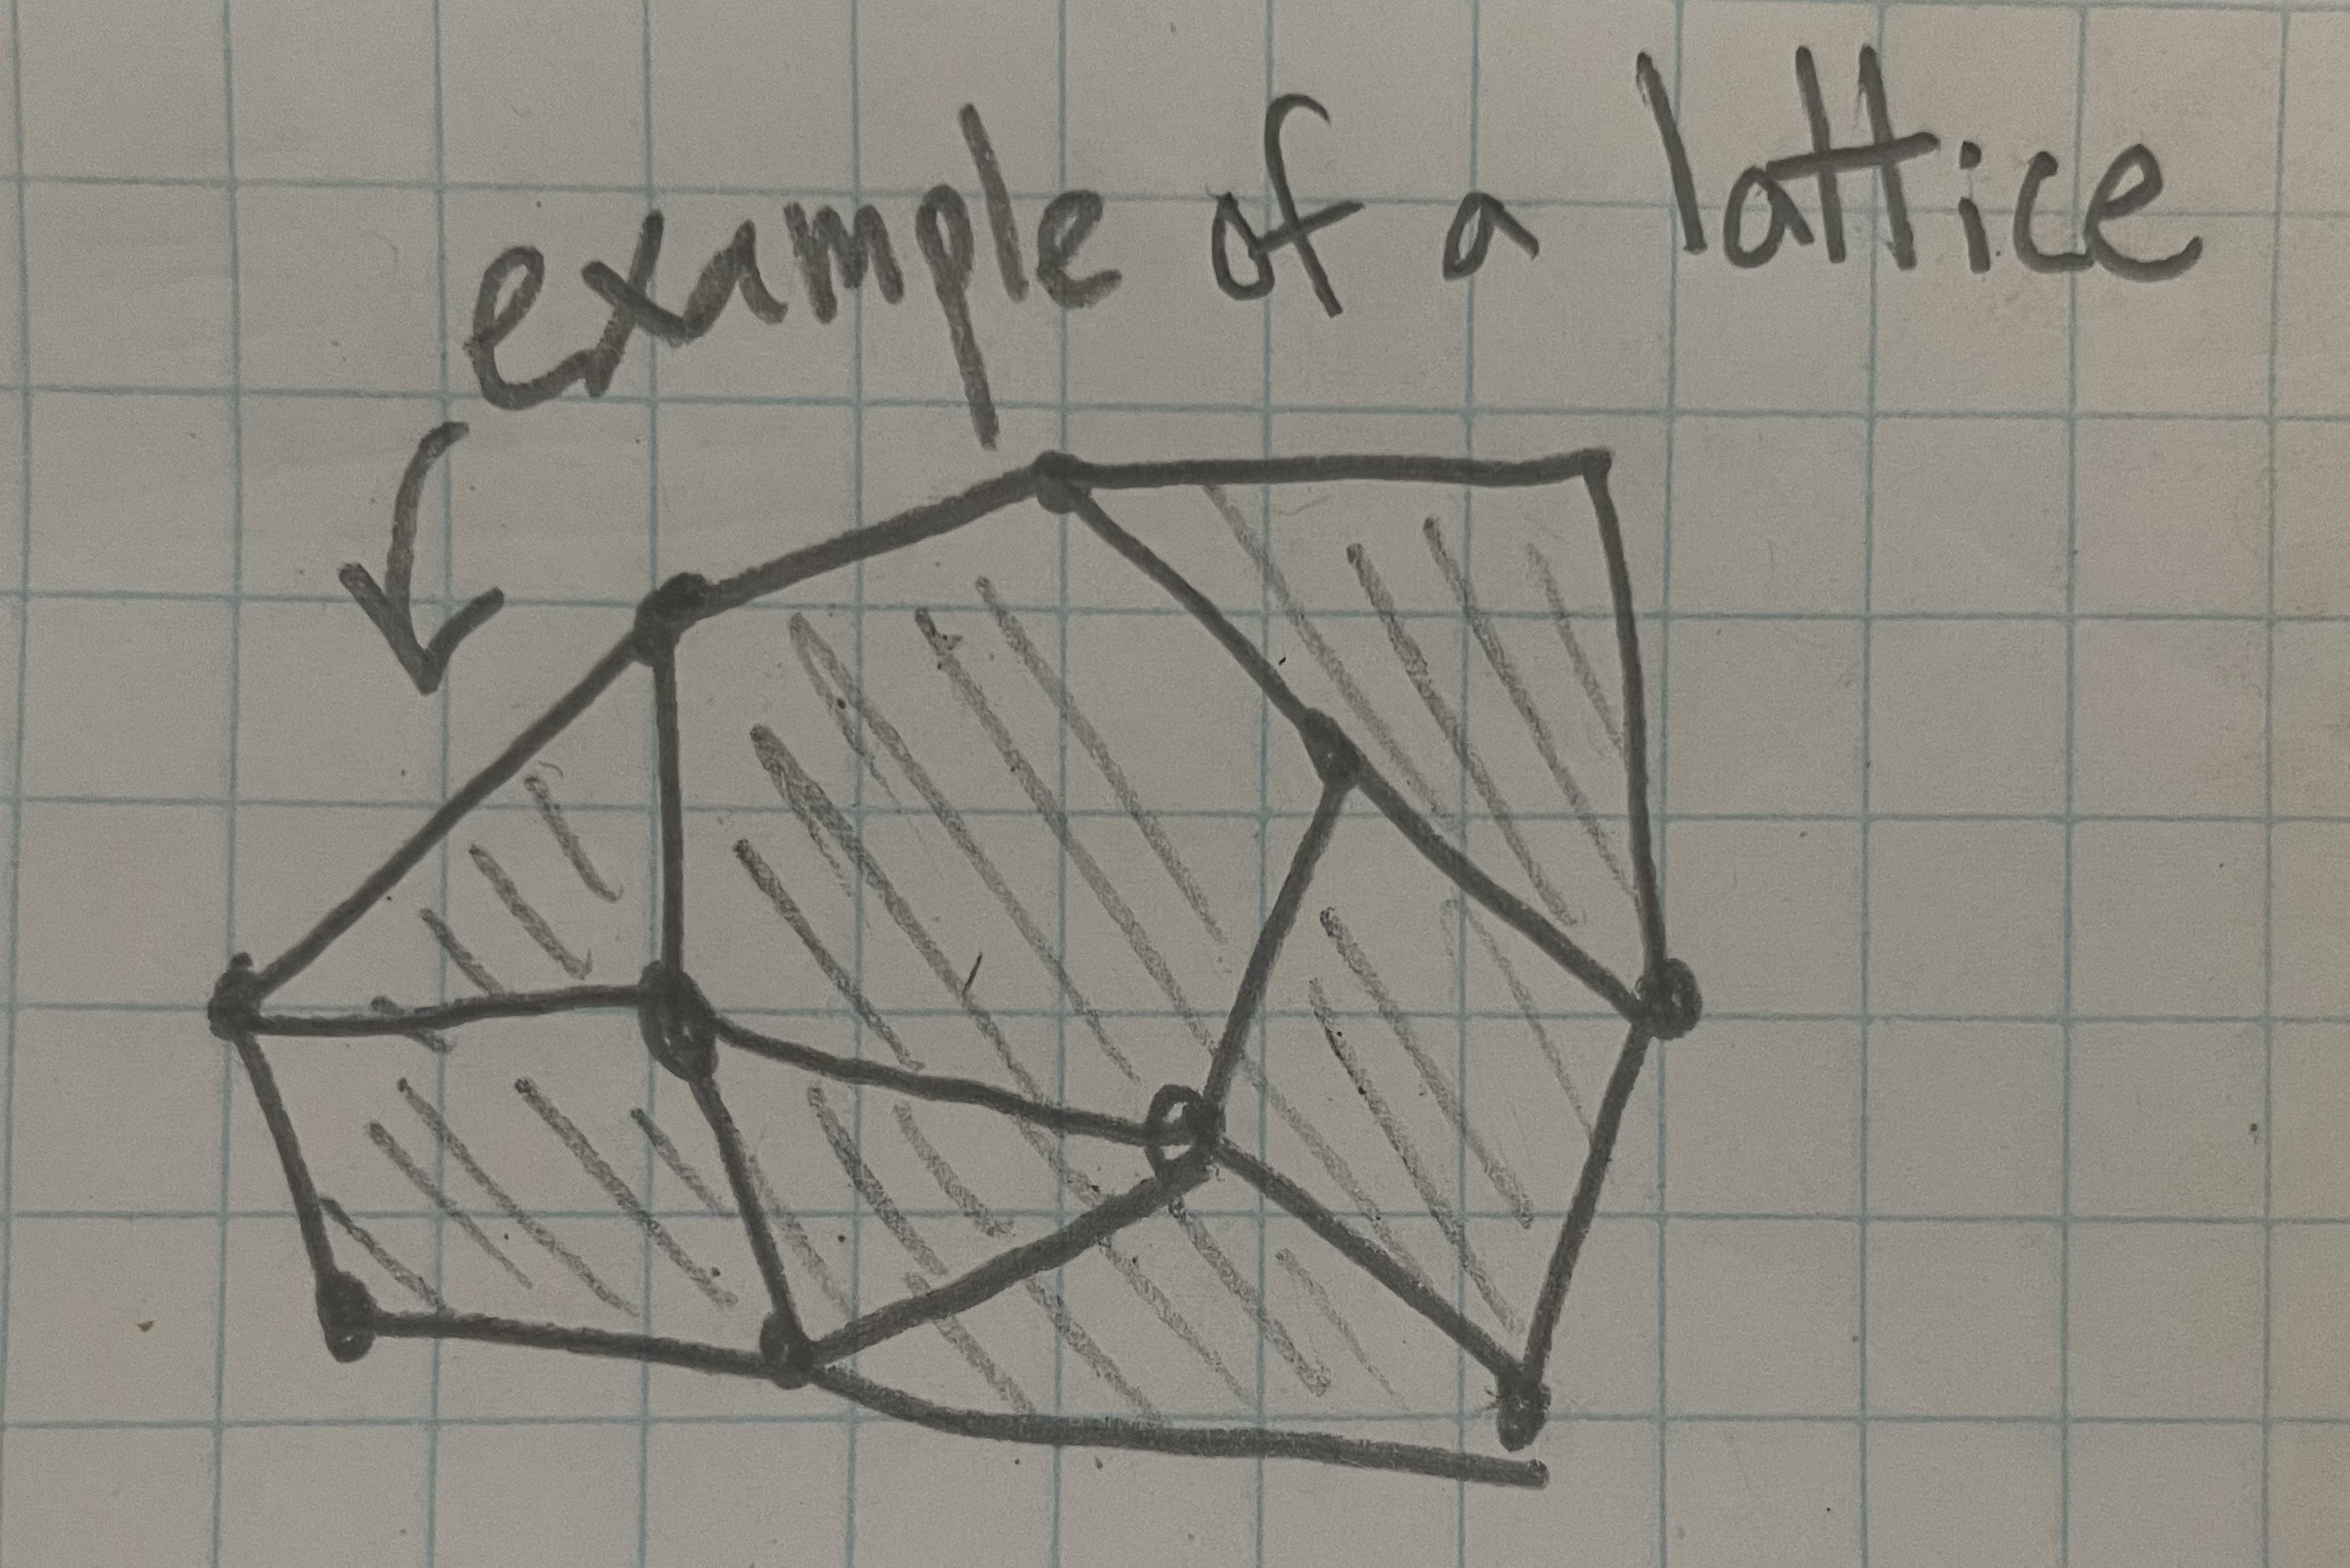
\includegraphics[scale=.04]{lattice-example}
\end{center}
\end{figure}

A lattice is a collection of vertices, edges, and faces connected in some way. To keep in line with the terminology common in topological quantum information, we refer to the faces of our lattices using the French term \textit{plaquette}. Formally, by lattice we mean ``simplicial 2-complex" though there is no need to go into details because we will never be dealing with the subtleties in the definition. Often times we will need to deal with \textit{directed} lattices. These are lattices in which every edge has a direction, which we represent as an arrow on that edge.

Before putting ordered media on a lattice, a good question is \textit{why} we would want to do this. There are two primary reasons. The first is that this will make this Hilbert spaces involved all finite dimensional. This is very important because we have only established quantum mechanics in the finite dimensional case, and working with the continuum limit can be highly complex. The second reason is that in practice, many of the systems physicists deal with are on lattices. For example, the chip of a quantum computer will store its information at finitely many sites, which can correspond to the vertices of some lattice. Many topological systems also arrise from materials which have crystal structures, which are modeled well by a lattice with atoms at the vertices and edges representing the geometry of the crystal.

The best setting for putting our ordered media on a lattice is by first putting on a torus. This helps for several reasons. Firstly, a torus is compact and hence it will add even more finiteness to the problem. Secondly, a torus has nontrivial topology which is useful for seeing the characteristic phenomina of topological order. Thirdly, a torus has no boundary, which helps because boundaries in topological order are subtle and require more work to describe. We denote the torus by $T^2$, and identify it with a square having its opposite sides glued:

\begin{figure}[h]
\begin{center}
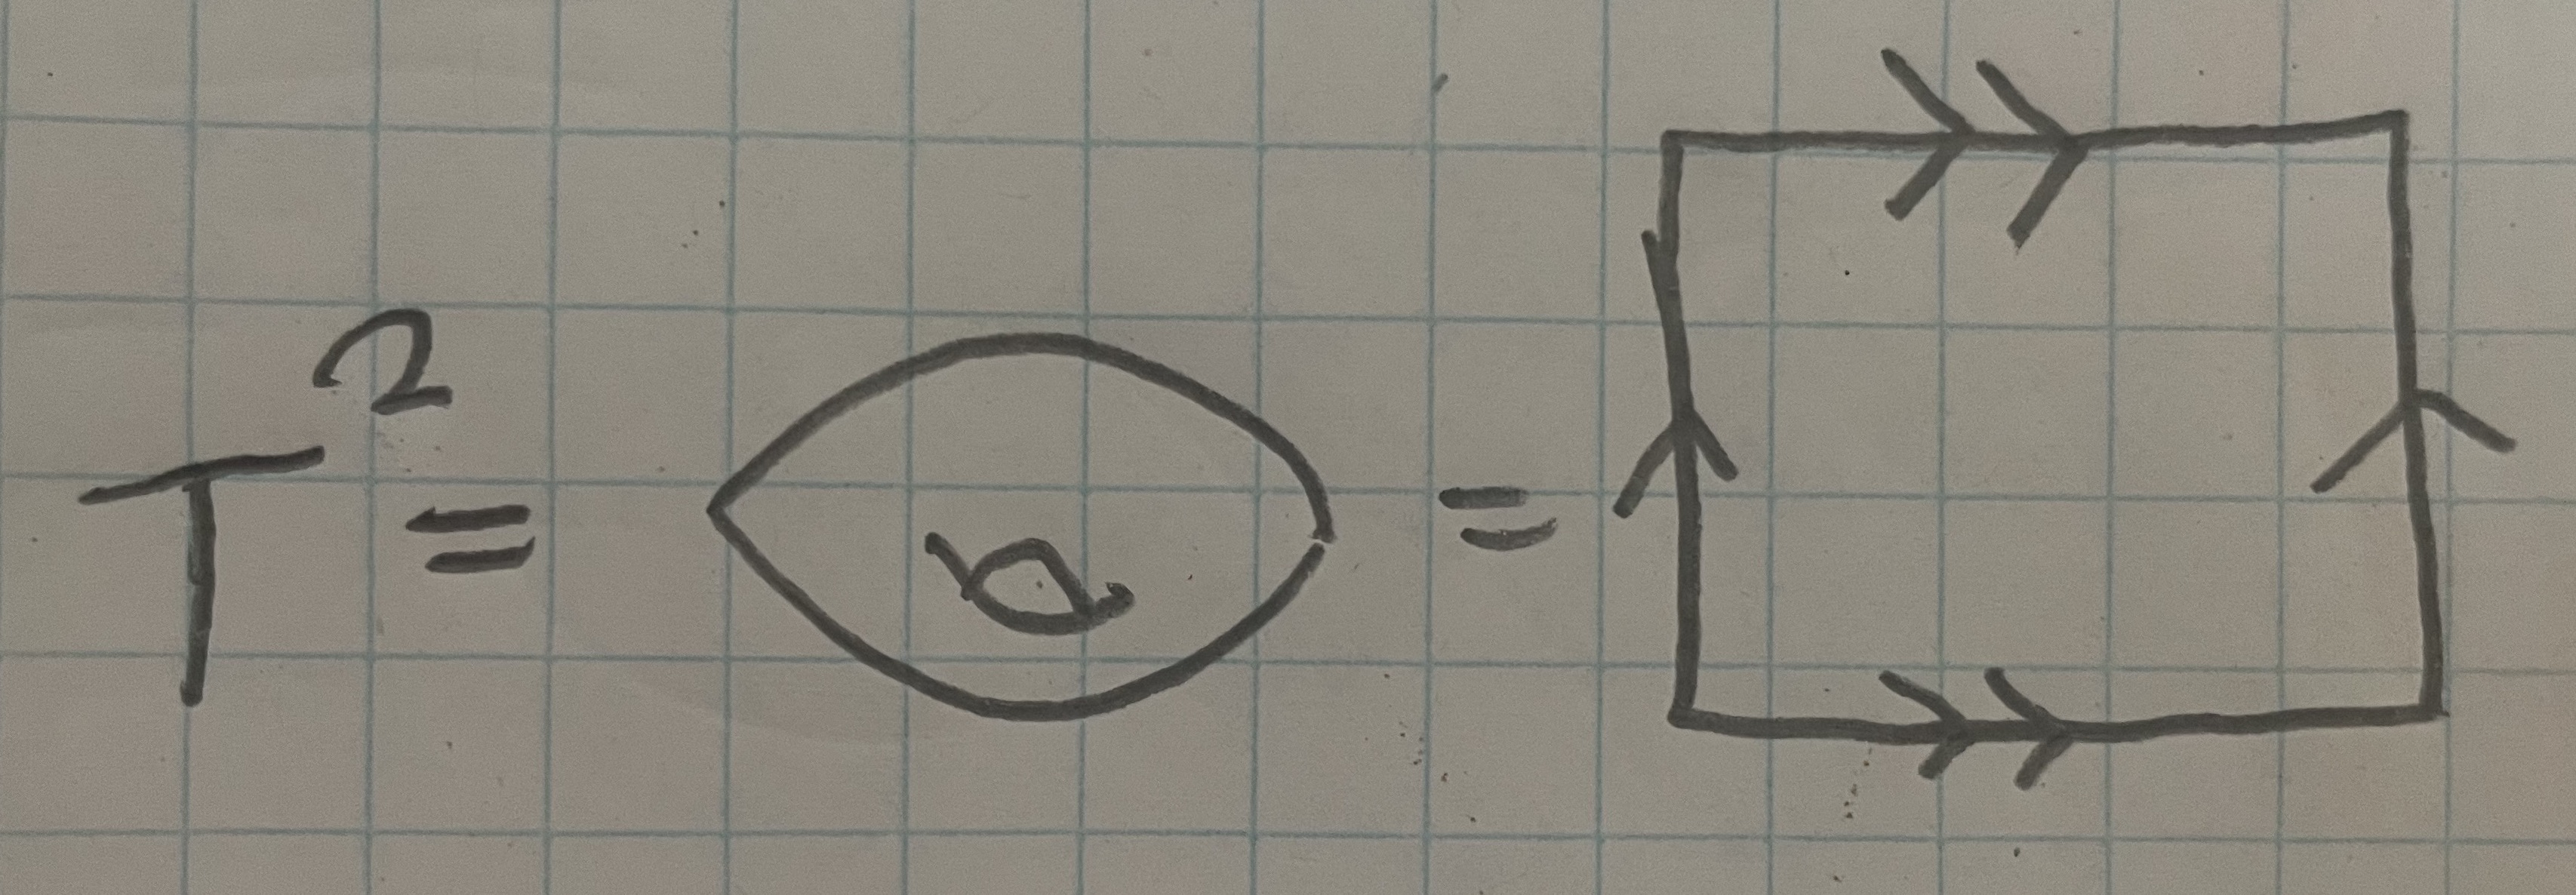
\includegraphics[scale=.04]{torus-definition}
\end{center}
\end{figure}

Ordered media on the torus corresponds to continuous maps $\phi: T^2\to M$ where $M$ is some fixed order space. The steps to transforming a state $\phi$ into a lattice version of itself go as follows:

\begin{enumerate}[Step $\text{1}$(a):]
\item Choose a directed lattice on the torus;
\item Choose a basepoint $m\in M$. Make \textit{local twists} around each vertex so that $\phi(v)=m$ for all vertices $v$ in the lattice.
\item On every edge, write down the winding number of $\phi$ along that edge, as an element of $\pi_1(M,m)$;
\item Forget $\phi$, and remember only the assignment of group elements in $\pi_1(M,m)$ to edges in the lattice.
\end{enumerate}

These steps deserve explanation. Step 1(a) is clear: we choose an arbitrary lattice on the torus. Typically we will choose the square lattice on the torus:

\begin{figure}[h]
\begin{center}
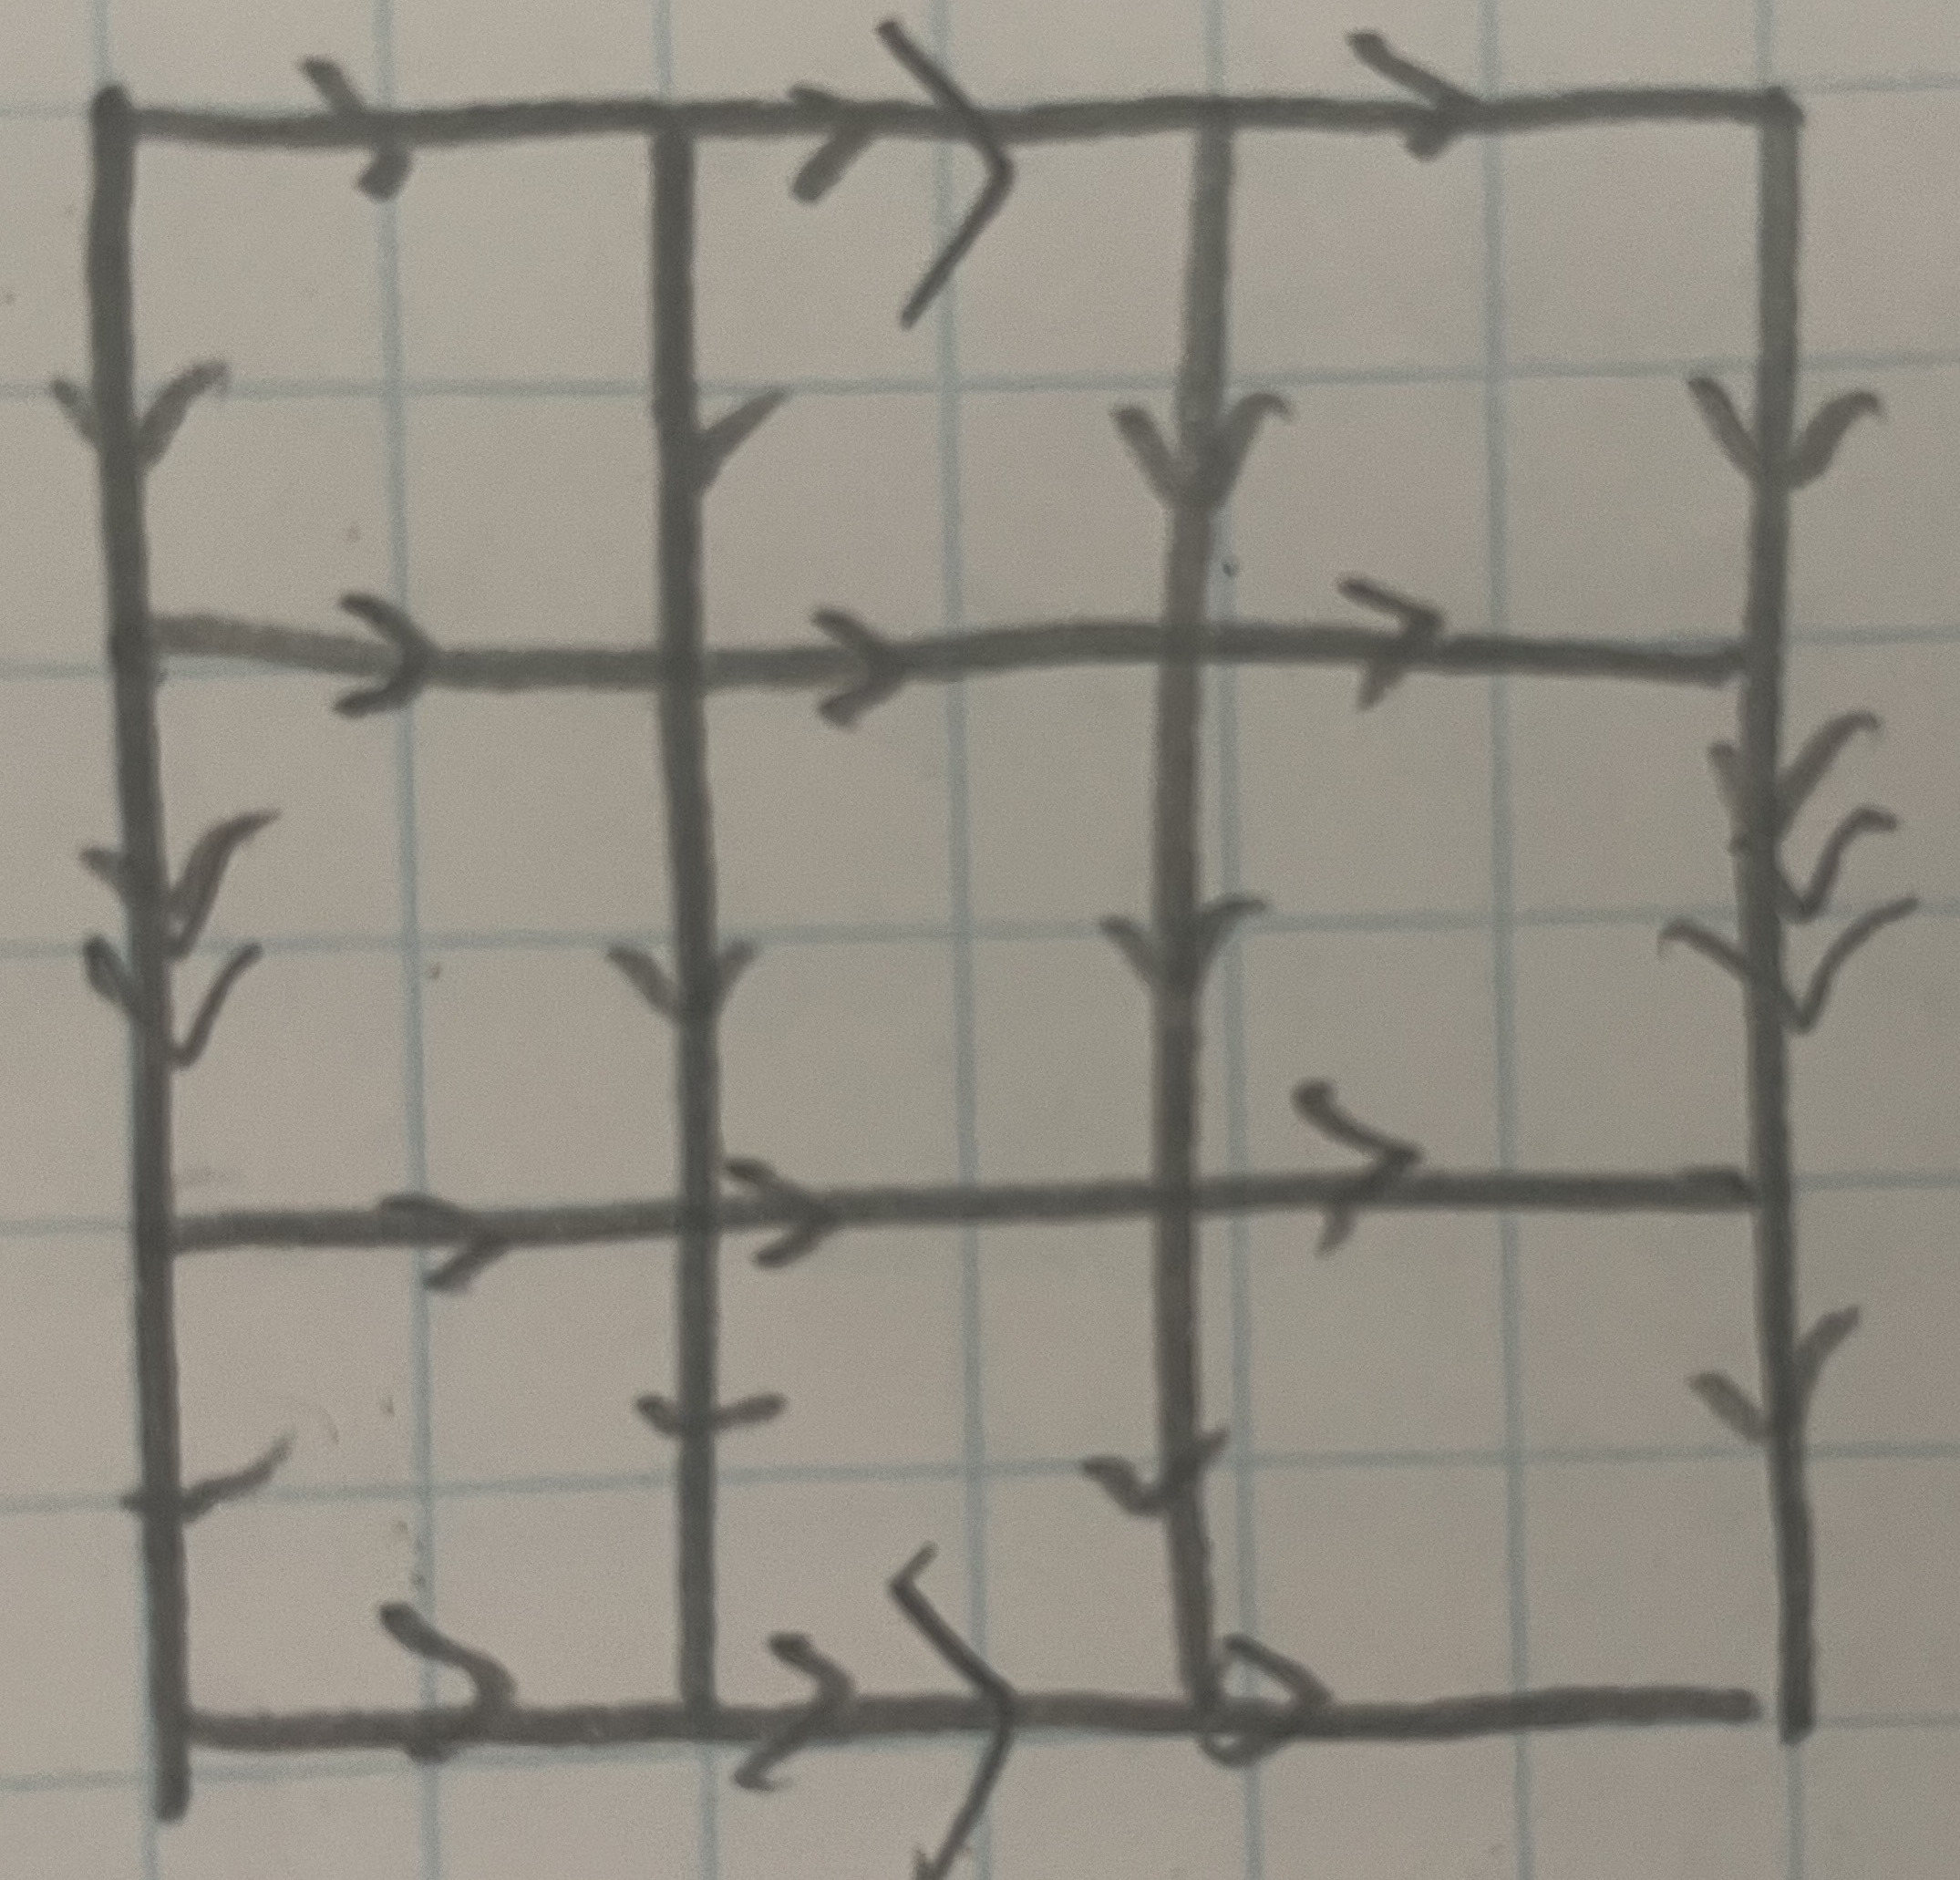
\includegraphics[scale=.04]{torus-lattice}
\end{center}
\end{figure}

Step 1(b) requires more explanation. The picture to imagine is that we take the state $\phi$ and twist its values in small neighborhoods around each vertex to enforce the condition $\phi(v)=m$. Formally, this means choosing another state $\tilde{\phi}$ such that $\tilde{\phi}(v)=m$ for every vertex $v$ of the lattice, and $\tilde{\phi}=\phi$ outside of some chosen small neighborhoods around each vertex. The fact that we can always choose such as state $\tilde{\phi}$ is a consequence of general mathematical principles in homotopy theory. Of course, different choices of $\tilde{\phi}$ will change the final result of our lattice encoding. However because any two choices of $\tilde{\phi}$ can only differ by local changes they can't be \textit{too} different, in a way we will quantify later in the subsection.

Step 1(c) is straightforward. Every edge can be thought of as a path. Pushing forward with $\phi$, this gives us a path in $M$. Since the edge starts and ends at vertices and $\phi$ sends all vertices to $m$, this means that the push forward of our edge gives a loop in $M$ based at $m$. Hence, it gives an element of $\pi_1(M,m)$. We can record this element and attach it as a piece of data associated to the edge.

Step 1(d) is entirely book keeping. It records the fact that we have successfully transformed our continuous data ($\phi:T^2\to M$) into discerete data (an assignement of group elements to edges in a lattice).

A worked example is shown below in the case that $M=S^1$ is the circle:

\begin{figure}[h]
\begin{center}
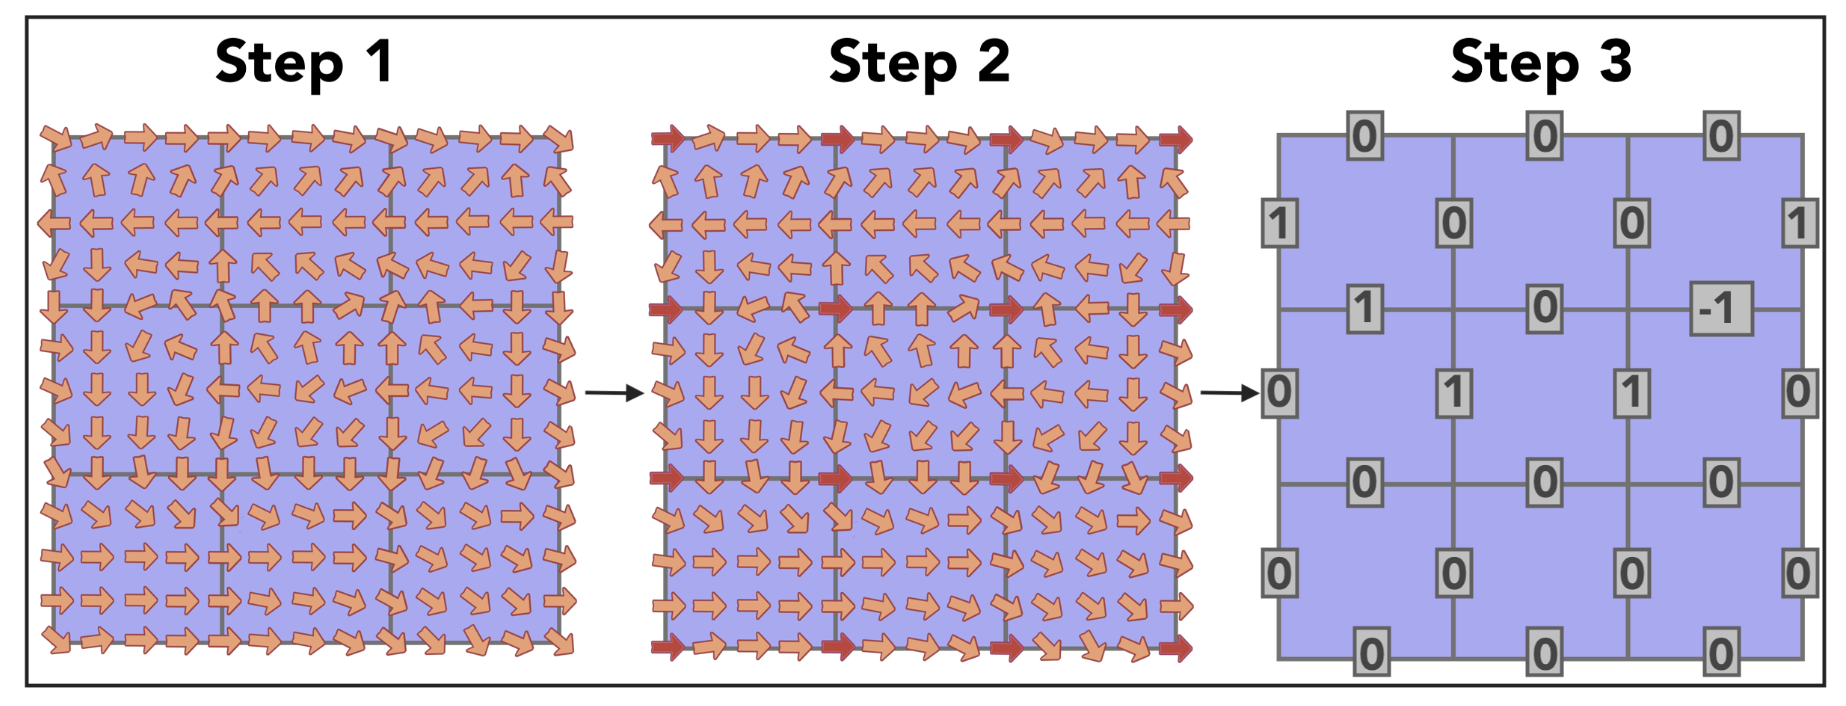
\includegraphics[scale=.3]{full-example}
\end{center}
\end{figure}

We now analyse our encoding of states in ordered media into assignements of group elements in $\pi_1(M,m)$ to edges in the lattice. The first fact from homotopy theory we will use is that these group elements determine the state $\phi$ exactly up to deformations localized within each face. Taking a limit of denser and denser lattices, this means that the group elements will specify $\phi$ up to increasingly local deformations. The intiution is that by taking an infinite lattice limit we should recover $\phi$ up to ``infinitely local deformations", i.e., we recover it exactly. In this way we did a good job with our lattice encoding.

We observe that not every assignement of group elements to edges appears in our construction. There are implicit conditions. In particular, imagine taking the product of the group elements on edges along some contractible loop, taking inverses appropriately so that all the arrows are pointing in the same direction. This product will be equal to the group element associated with the loop around this whole path. The winding number along any contractible path under a continuous map should be trivial. Hence, the product of these group elements should be trivial. In particular, given any plaquette, the ordered product of group elements along its edges should be zero:

\begin{figure}[h]
\begin{center}
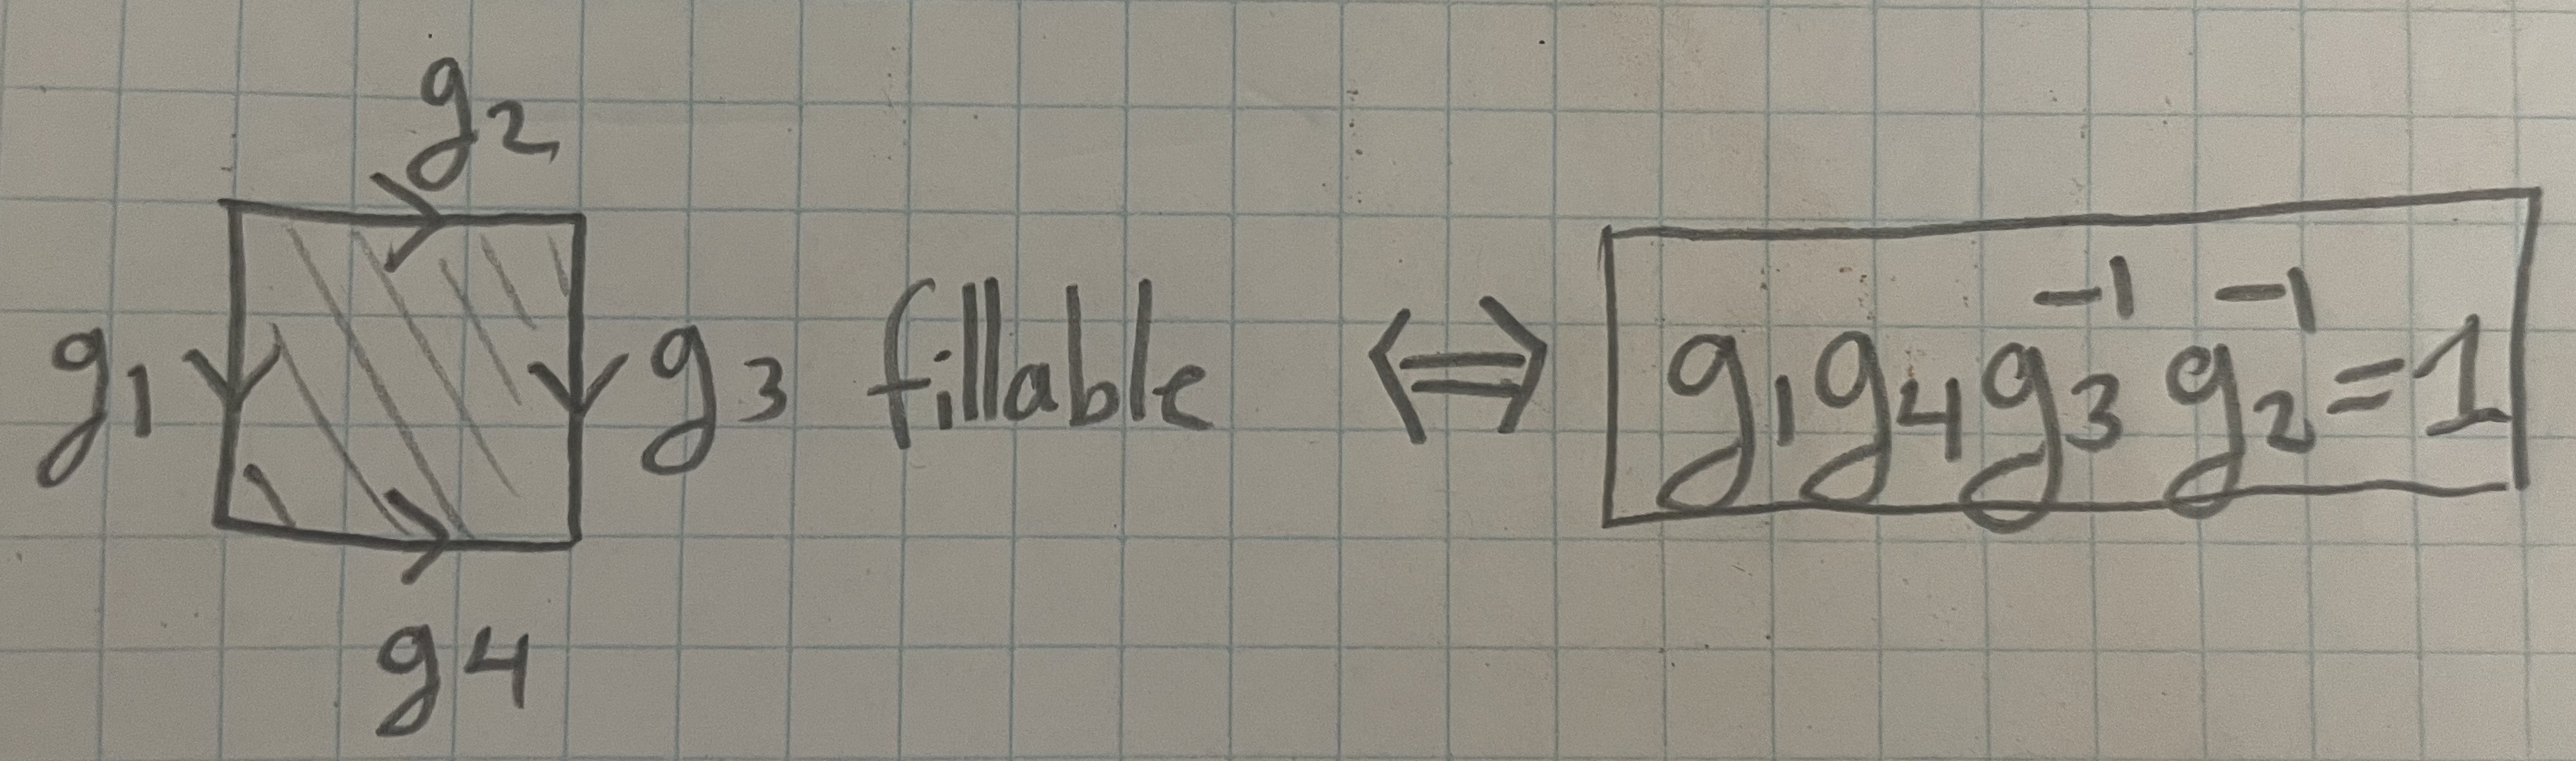
\includegraphics[scale=.06]{plaquette-rule}
\end{center}
\end{figure}

Moreover, \textit{any} coloring of the edges of the lattice by elements of $\pi_1(M,m)$ will come from some map $\phi$ so long as it satisfies the condition above. This is one of the key formulas of the theory. It is in a real sense a lattice version of the continuity condition, since it is \textit{equivalent} to the condition of continuity in the infinite lattice limit. This lattice version of continutity is called \textit{flatness}. Flatness conditions are the most common sort of compatibility conditions which appear when you have local degrees of freedom valued in some group, making this lattice situation very general.

The last thing do deal with in analysing our system is deformation. When analysing states in ordered media, a huge amount of our time was spent on performing continuous deformations. Topological information is defined to be information which is invariant under continuous deformation. What does this correspond to in the lattice model?

Suppose we are given an ordered media state $\phi$ and its corresponding lattice coloring. If we deform $\phi$ in some small neighborhood within a face, this will not change the values along the edges and hence will not change the coloring. If we deform $\phi$ in some small neighborhood around the interior of some edge this also won't change the coloring, because this will correspond to deforming the loop in $M$ induced by going along that edge, and elements of the fundamental group are invariant under deformations of this sort. Another way of seeing that the coloring can't change is that flatness must be preserved - if the group element on the deformed edge changed, it would ruin flatness on the faces it bounds.

Finally, we can consider deforming $\phi$ around some vertex. This certainly \textit{can} impact the coloring. An easy way to compute how it must impact the coloring is by using the fact that the flatness condition must be preserved. Suppose that an incoming edge labled by $g_1$ changes to $g_1 g$ after the deformation. Enforcing flatness along all of the faces touching the vertex allows one to conclude that all incoming edges $g_k$ will get changed to $g_k g$, and all outgoing edges $g_k$ will get changed to $g^{-1}g_k$, as shown below:

\begin{figure}[h]
\begin{center}
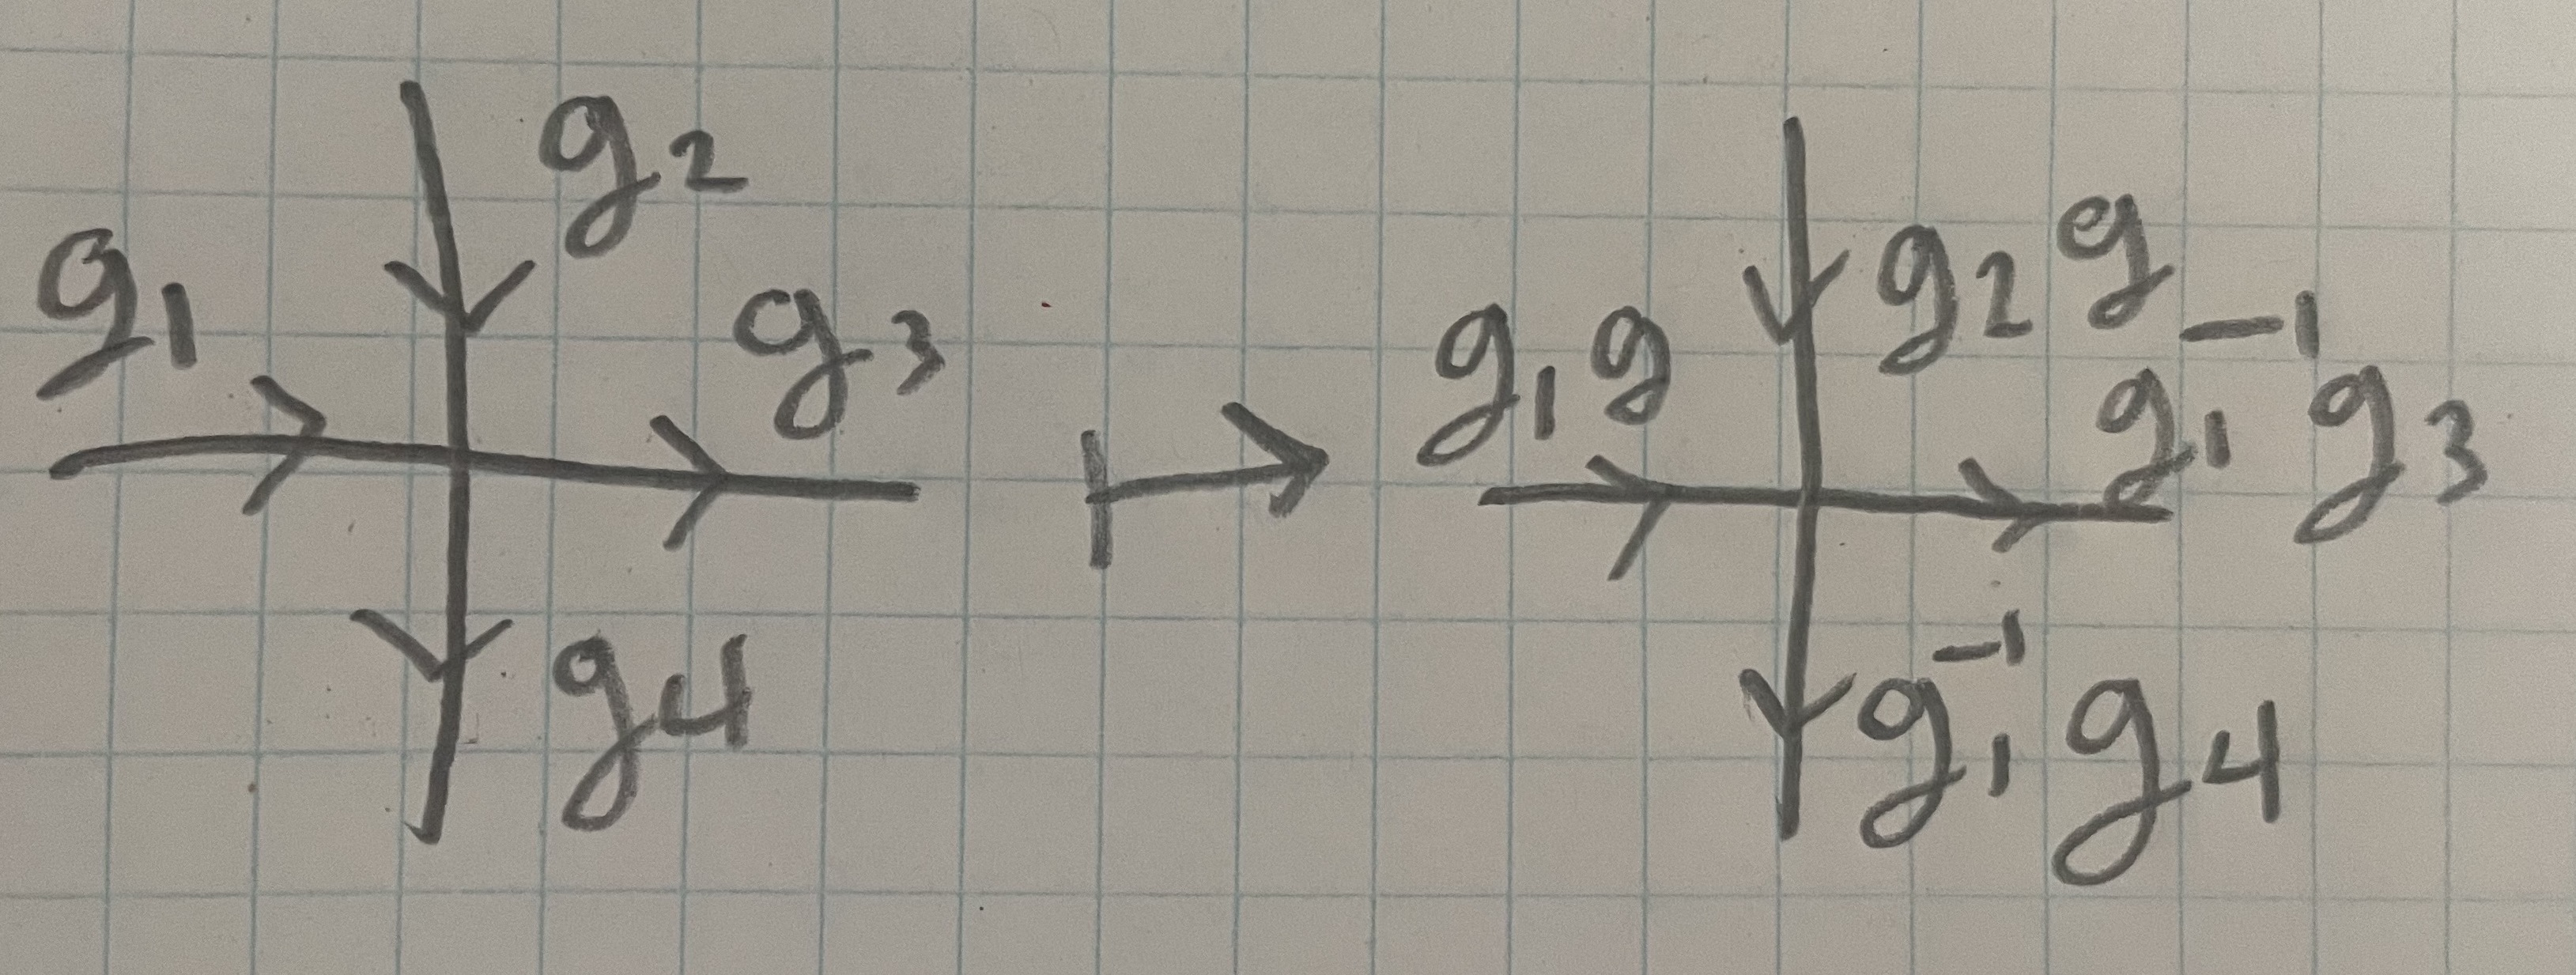
\includegraphics[scale=.04]{gauge-transformation}
\end{center}
\end{figure}

Another way of seeing this result is by anlysing what a deformation of $\phi$ does. The value $\phi(v)$ can move along some loop, starting and ending at $m$. This loop induces some element of the fundamental group, $g\in \pi_1(M,m)$. Performing this deformation exactly acts by precomposing/postcomposing the adject edges with $g$/ $g^{-1}$ accordingly. We can see below a concrete example for $G=S^{1}$:

\begin{figure}[h]
\begin{center}
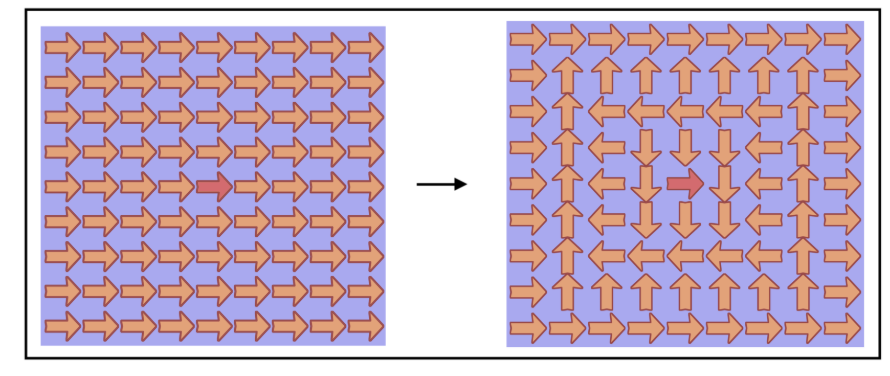
\includegraphics[scale=.45]{twisting}
\end{center}
\end{figure}

Hence, we have a picture for ordered media on the lattice: states correspond to flat colorings of elements of $\pi_1(M,m)$ on a fixed lattice, and continuous deformations correspond to certain vertex actions by elements of $\pi_1(M,m)$.

\subsubsection{From ordered media to gauge theory}

In the previous subsection we showed how to put ordered media on a lattice. In this section we show how to make it quantum, turning it from a classical field theory to a quantum gauge theory. The idea of this jump is as follows. In Section [ref] we obtained an equivalence

$$
\left(\substack{\text{topological information}\\ \text{in ordered media}}\right)=\left(\text{states}\right)/\left(\substack{\text{continuous} \\ \text{deformation}}\right).
$$

It is neccecary to mod out by continuous deformation because there is topoloigcal information in states, but also local degrees of freedom. For instance, the group element assigned to any indivudal edge in ordered media on a lattice can be changed by a gauge transformation and hence is not topologically invariant. The idea of going from ordered media to gauge theory is as follows: gauge theory is what results from ordered media when quantum fluxtuations become so strong that local degrees of freedom are completely washed out and only the topology remains.

The fluxtuations are quantum because we will imagine that our states will evolve in such a way that they are in a superposition of gauge transformations having been applied and not having been applied. Our states in gauge theory will be \textit{equal superpositions over all possible deformations} of a given state. In this way, we are using quantum mechanics as a physical mechanism for quotients. Equivalence classes under deformation will be physically realized as equal superpositions over all possible representatives.

This can all be made completely rigorous. Choose a lattice on the torus, an order space $M$, and a basepoint $m$. We define a Hilbert space

$$\cN=\bigotimes_{\text{edges}}\bC[G].$$

We canonically identify the standard basis of $\cN$ with $G$-colorings of the lattice. Let $C$ be an equivalence class of flat $G$-colorings of $\cN$ up to gauge transformations. There is a corresponding state

$$\ket{C}=\sum_{\gamma \in C}\frac{1}{\sqrt{|C|}}\ket{\gamma}.$$

This state is a normalized equal superposition of representatives of $C$. This defines a sub-Hilbert space

$$\bC=\text{span}\left\{\left.\ket{C}\right| C\in \text{(flat $G$-colorings)}/\text{(gauge transformations)}\right\}.$$

This Hilbert space $\bC$ stores the information in our gauge theory.

So far our system is relatively trivial - it is just a Hilbert space, with no Hamiltonian. We connect it back to our original picture of topological order. The space $\bC$ is the collection of ground states in a topologically ordered system. Above it there is a whole spectrum of other states. This fuller picture with a Hamiltonian adds all of the subtlety and intrigue to the system.

In particular, we observed in Chapter [ref] section [ref] we observed the importants of quasiparticles in ordered media. These formed the heart of our information processing. Similarly, in gauge theory there will be quasiparticles as well which appear higher up in the spectrum of the Hamiltonian. Some of these quasiparticles will correspond to the classical quasiparticles in ordered media, but others are entirely new features of the system which did not exist before. We will analyse all this in more in the subsection that follows.

\subsubsection{Kitaev quantum double model}

[WORK: not sure if this is readable to someone who skipped the first two sections, but it should be. Something to keep an eye on.]

[WORK: Use $\fD(G)$ as notation for the doubled quantum order associated to $G$.]

In this section we will give the Hamiltonian formulation of discrete gauge theory. Seeing as we have moved passed ordered media, we will no longer be working with order spaces and base points. Instead, we will choose an abstract finite group $G$ which replaces $\pi_1(M,m)$. The general picture for creating our Hamiltonian is simple, and follows a very general pattern in quantum theory: instead of enforcing properties rigidly as conditions, we will enforce them enforce properties energetically as terms in a Hamiltonian. The formulation we give below is known as the \textit{Kitaev quantum double model of discrete gauge theory}. It was introduced in Kitaev's seminimal paper on topological quantum information [ref]. It has been studied extensively in the literature by many authors [add more refs].

Choose a directed lattice on the torus. Let

$$\cN=\bigotimes_{\text{edges}}\bC[G]$$

be the HIlbert space of our quantum system. The space $\cN$ has a canonical basis given by $\prod_{\text{edges}}G$, which we  identify with $G$-colorings of the lattice. Given a $G$-coloring $\gamma$, we will denote the corresponding state in $\cN$ by $\ket{\gamma}$. For every plaquette $p$ in the lattice, we define an operator on $\cN$ by

$$B_p\ket{\gamma}=
\begin{cases}
\ket{\gamma} & \gamma \text{ flat at }p\\
0 & \text{otherwise}.
\end{cases}$$

We observe immediately that

$$\sum_{\text{plaquettes }p}(1-B_p)\ket{\gamma}=0 \iff \ket{\gamma} \text{ is flat.}$$

It is in this way that we can enforce properties energetically by adding them as terms to a Hamiltonian. If we chose the Hamiltonian to be $\sum_{\text{plaquettes }p}(1-B_p)$, then the lowest energy eigenspace would exactly correspond to the space spanned by flat $G$-colorings. For every vertex $v$ and group element $g\in G$, we define an operator on $\cN$ by

$$A_{v,g}\ket{\gamma}=\ket{\gamma \text{ acted on by the $g$ gauge action at $v$}}.$$

For any $\ket{\psi}\in \cN$, we call $\ket{\psi}$ \textit{gauge invariant at $v$} if $A_{v,g}\ket{\psi}=\ket{\psi}$ for all $g\in G$. We call $\ket{\psi}$ gauge invariant if it is gauge invariant at $v$ for all vertices $v$. We define

$$A_v=\frac{1}{|G|}\sum_{g\in G}A_{v,g}.$$

We define the Hamiltonian of our system to be

$$H=\sum_{\text{vertices $v$}}(I-A_v)+\sum_{\text{plaquettes $p$}}(I-B_p)$$

where $I$ is the identity operator. We summarize the basic properties of this Hamiltonian below:

\begin{prop} The following properties of the Kitaev quantum double Hamiltonian hold:

\begin{enumerate}[(a)]
\item The operators $A_v$, $B_p$, and $H$ are Hermitian for all vertices $v$ and plaquettes $p$;
\item The formula $A_{v,g}^{\dagger}=A_{v,-g}$ holds for all vertices $v$ and $g\in G$;
\item All of the operators in the set $\{A_v,B_p\}_{v\in \text{vertices}, p\in \text{plaquettes}}$ commute with every other operator in the set;
\item The eigenstates of $H$ are simultaneous eigenstates of the operators $A_v$, $B_p$;
\item The eigenvalues of the $A_v,B_p$ are all $0$ or $1$;
\item The lowest eigenvalue of $H$ is $0$, and the $0$-eigenspace of $H$ is

$$\bC=\text{span}\left\{\left.\ket{C}\right| C\in \text{(flat $G$-colorings)}/\text{(gauge transformations)}\right\}.$$

where for we define the ket

$$\ket{C}=\sum_{\gamma \in C}\frac{1}{\sqrt{|C|}}\ket{\gamma}$$

for any equivalence class $C$ of $G$-colorings of the lattice up to gauge transformations.

\end{enumerate}
\end{prop}
\begin{proof}.[WORK: do proof]
\end{proof}

In particular, the above proposition tells us exactly that we have acheived our goal of realizing a Hamiltonian whose ground states capture the topological information in a lattice-version of ordered media.  The term ``double" in the Kitaev quantum double model refers to the fact that there are two families of terms in $H$ - one family of type $A_v$ and one family of type $B_p$. We can readily compute the dimension of the ground space as follows:

\begin{prop} Choose a vertex $v$ in the lattice. Every $G$-coloring of the lattice induces an assignment of lattice loops on the torus based at $v$ to elements of $G$, based on taking the oriented winding number along that loop relative to the coloring. This restricts to a map

$$(\text{flat $G$-colorings})\xrightarrow{}\Hom(\pi_1(T^2,v), G)$$

where $\Hom(\cdot,\cdot)$ denotes the space of group homomorphisms between two groups. Any two flat $G$-colorings which differ by gauge transformations will induce the same map in $\Hom(\pi_1(T^2,v), G)$, up to global conjugation by an element of $G$. This induces a bijection

$$(\text{flat $G$-colorings})/(\text{gauge transformations})\xrightarrow{}\Hom(\pi_1(T^2,v), G)/\left(\substack{\text{simultaneous} \\ \text{conjugation}}\right).$$

The set of vectors ${\ket{C}}_{C\in (\text{flat $G$-colorings})/(\text{gauge transformations})}$ is linearly independent. Hence, there is a canonical isomorphism

$$\bC \xrightarrow{}\bC[\Hom(\pi_1(T^2,v), G)/\left(\substack{\text{simultaneous} \\ \text{conjugation}}\right)]$$

given by taking winding numbers.
\end{prop}
\begin{proof}.[WORK: give proof. I'm scared this could be too hard. It's already]
\end{proof}

The final step in using the above formula is to compute the fundamental group of the torus:

\begin{prop} $\pi_1(T^2,v)\cong \bZ^2$ for any vertex $v$. The two loops shown below are generators for $\pi_1(T^2,v)$:

\begin{figure}[h]
\begin{center}
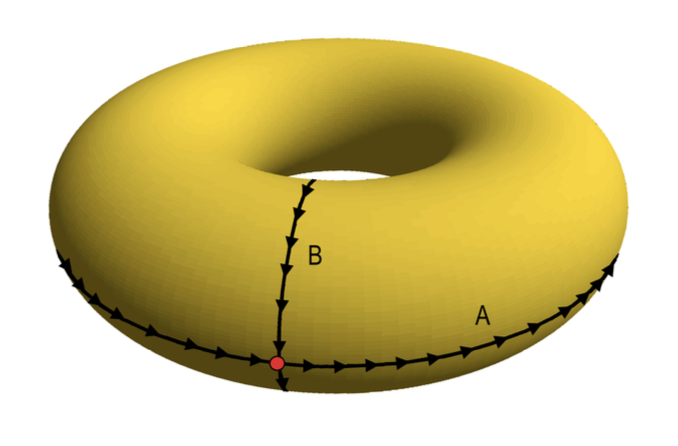
\includegraphics[scale=.3]{torus}
\end{center}
\end{figure}

\end{prop}
\begin{proof}.[WORK: proof]
\end{proof}

One last observation to make about this ground space is that its ground states really are globally different:

\begin{prop} Let $L$ be length of the shortest non-contractible loop on the lattice. Let $\gamma_0,\gamma_1$ be non-gauge equivalent flat $G$-colorings of the lattice. There are at least $L$ edges at which $\gamma_0$ and $\gamma_1$ assign different values.
\end{prop} 
\begin{proof}.[WORK: do proof]
\end{proof}

In particular, if we choose the square lattice on the torus, then the length $L$ of the shortest non-contractible loop is obvioulsy a good measure of linear system size. Proposition [ref] tells us that the number of local changes requires to go from one ground state to another is on the order of $L$. This is exactly the sort of condition we needed in Section [ref] to conclude topological protection in the ground states. Of course, the smallest non-zero eigenvalue of $H$ is at least $1$, which is bounded away from zero and hence there is a system-size independent gap between the ground states and the other states. Hence, we see that $H$ is a good topologically ordered Hamiltonian. 

The excited states of $H$ will be described localized excitations with quasiparticle behavior. Given a state $\ket{\psi}\in \cN$, we will say that a state has an \textit{excitation at vertex $v$} if $A_v\ket{\psi}=0$ and we will say that is \textit{unnoccupied at $p$} if $A_v\ket{\psi}=1$. We say that $\ket{\psi}$ has an \textit{excitation at plaquette $p$} if $B_p\ket{\psi}=0$ and that it is \textit{unnocupied at $p$} if $B_p\ket{\psi}=1$. By Proposition [ref], every energy eigensate is either occupied or unoccupied at every vertex/plaquette. The regions in which $\ket{\psi}$ is unnoccupied are all essentially identical, leading to a homogenous bulk. The sites at which $\ket{\psi}$ is occupied are different, and behave as quasiparticles. We will define operators which move these excitations around.

[WORK: Add something about local indistinguishability of ground states - reinforce this ``homogenous bulk" idea.

More than this, it is important to note that earlier we are giving a rigorous definition of topological order. It is not immediately obvious that the KQDM satisfies this definition. This is the main content of the paper \cite{cui2020kitaev}. Should I include a proof? At the very least there should be some mention of how this fits into the definition. In fact, this should be a big point. The KQDM is being introduced with the main goal of giving an example of TO. Needs to talk about how it is topological.]

[WORK: Maybe also reinforce that this could be done on \textit{any manifold}, and the gound states would be the same? ]

\subsection{The toric code}

[WORK: Maybe this section can be re-done. We know that the total space $\cN$ can be decomposed as a direct sum

$$\cN=\bigoplus_{\lambda}\cN_\lambda$$

as a direct sum over syndromes, by general principles of diagonalizable matrices. To prove that all of the $\cN_\lambda$  have an even $\#$ of excited terms in $H$ of both $A_v$ and $B_p$ type is easy. Proving that they all have the same dimension involves the simple observation that applying $\sigma_X$ and $\sigma_Z$ between two excited terms will make them both ground states. Simple counting recovers the fact that the ground state is $4$-dimensional.

The beauty of this approach is that it is immediately grounded. We have a Hamiltonian, we want to solve it - i.e. we want to compute the dimensions of the $\cN_\lambda$, and explicitely have a way of creating those basis states. The proof in a real sense is using the quasiparticle nature of the $A_v$ and $B_p$ excitations. Namely they are being moved along paths to annhilate with one another.

Every operator can be decomposed as a sum of Pauli operators. Hence, unerstanding how Paulis act on $\cN$ lets understand how every operator acts on $\cN$. Paulis act on $\cN$ by creating/moving/fusing vertex/plaquette excitations. Hence, understanding vertex/plaquette excitations tells you everything you need to know about the toric code. Saying it this way makes everything feel very grounded, and it doesn't bring in anyons unnececarily early into the picture. We can talk about anyons after. Highlight the fact that they behave like quasiparticles and that they will become objects of independent interest, but that isn't the point yet.

]

\subsubsection{Simplified Hamiltonian}

In this section we move on to analyzing the Kitaev quantum double model for $G=\bZ_2$, which is known as the \textit{toric code}. The name toric code comes from the fact that the toric code was first introduced as an error correcting code, and was only later recast as a topologically ordered system [refs]. The toric code is still the basis for many of the most popular error correcting codes [refs]. In a real sense the toric code is the simplest nontrivial topological order. It is a fantastic example which demonstrates almost all of the phenomina of topological order with relatively little work involved. The toric code, and more generally $\bZ_2$ discrete gauge theories, can be found in all sorts of systems such as [WORK: give examples. The ones that jump to mind are dimer models - \cite{moessner2001resonating, misguich2002quantum}]. 

We describe the model now. Because $G=\bZ_2$ is abelian, we will switch to additive notation for our group operation. We choose a \textit{non-oriented} lattice structure on the torus. This lattice does not need to be oriented because changing the direction of edges in the lattice corresponds to taking inverses, and $g=g^{-1}$ for every element $g\in \bZ_2$. We define

$$\cN = \bigotimes_{\text{edges}}\bC[\bZ_2]=\bigotimes_{\text{edges}}\bC^2.$$

Here, we identify $\bC[\bZ_2]$ with $\bC^2$ for convenience, endowing $\bC^2$ with a canonical basis $\{\ket{0},\ket{1}\}$. We call $\bC^2$ a \textit{qubit}, in analogy to ``bits" for classical computing. It is a standard two-level quantum system. Most quantum computers are based on qubits, which makes the toric code especially accessable to practical implementation as an error correcting code. The definition of the Hilbert space $\cN$ can be summarized as putting a qubit on every edge of the lattice. The Hamiltonian is

$$H=\sum_{\text{vertices }v}(1-A_v)+\sum_{\text{plaquettes }p}(1-B_p).$$

We unpack the general definitions of $A_v$ and $B_p$ for the toric code. The operator $A_{v,0}$ is the identity. The operator $A_{v,1}$ acts by a gauge transformation,

\begin{figure}[h]
\begin{center}
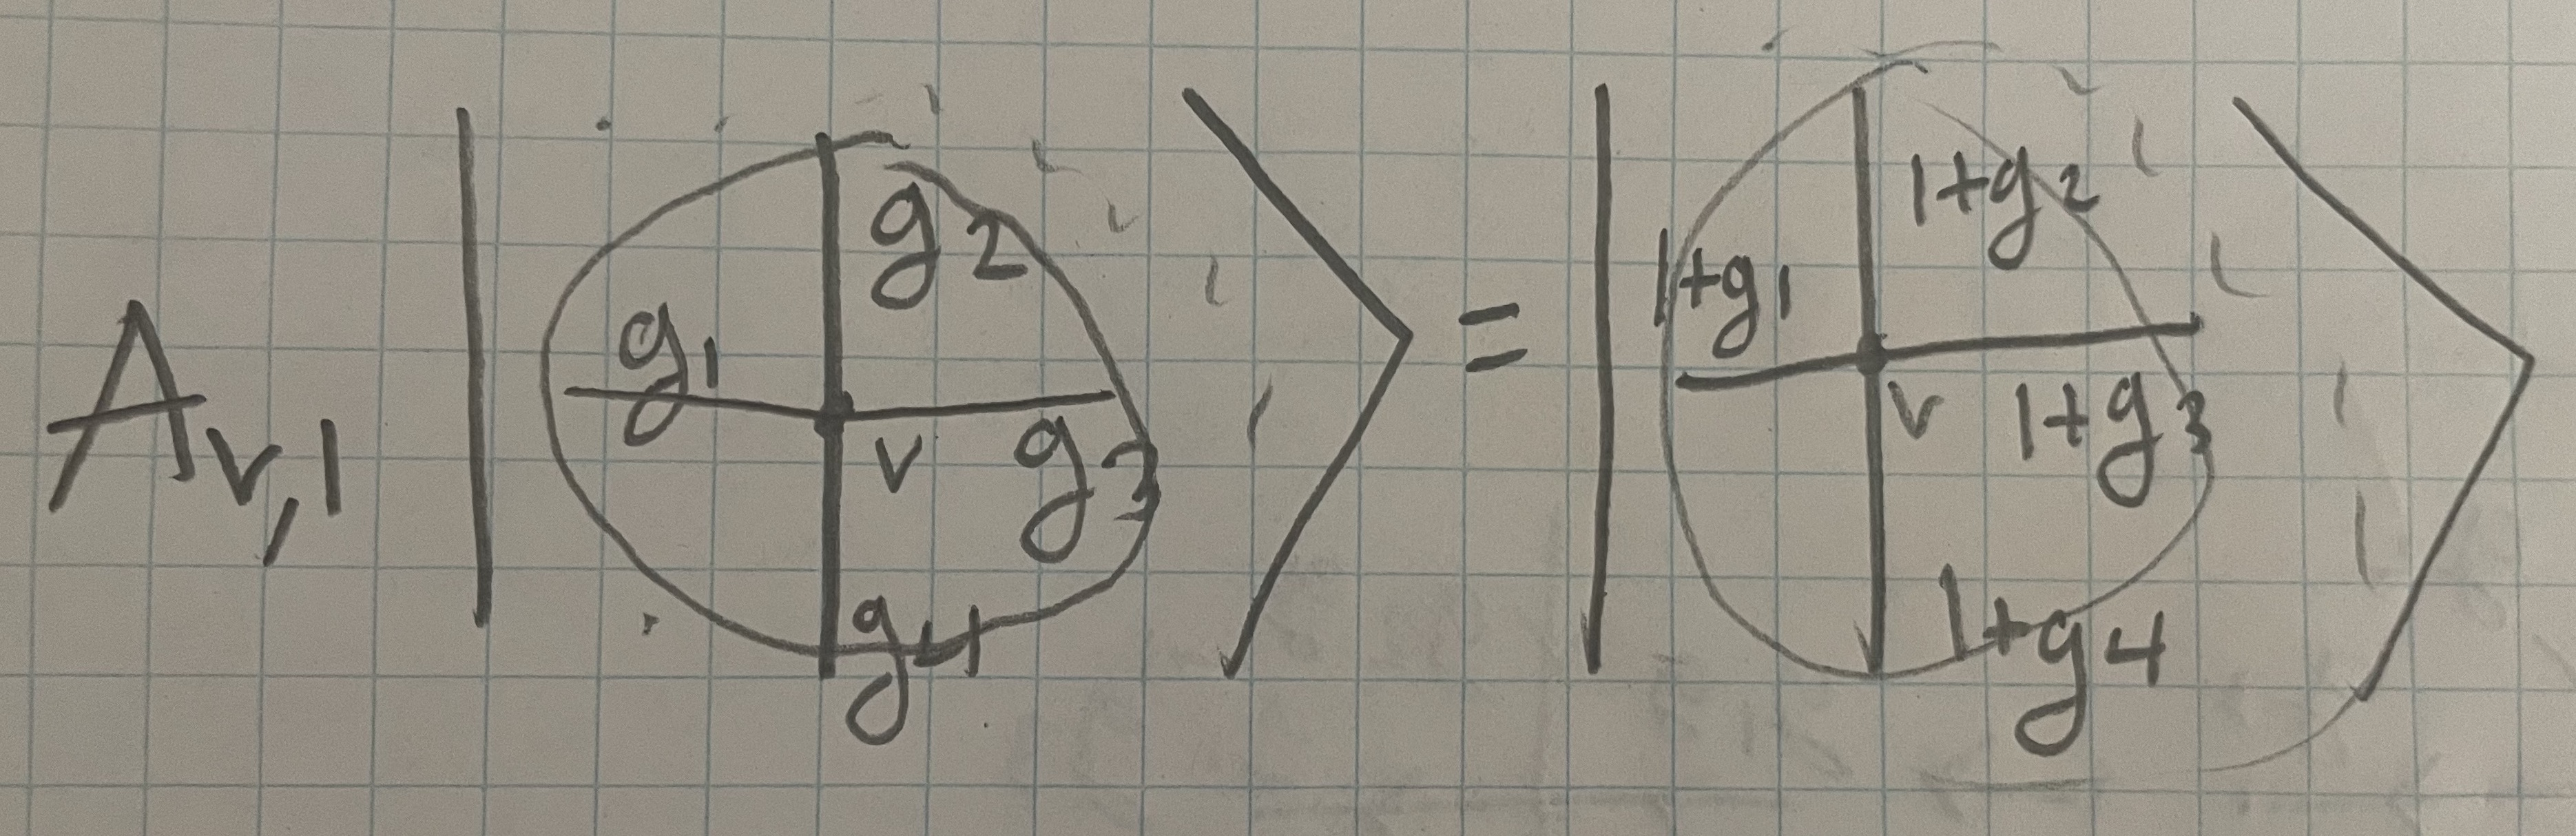
\includegraphics[scale=.04]{Av-gauge-action}
\end{center}
\end{figure}

Defining

\begin{align*}
\sigma_X:\bC^2&\xrightarrow{}\bC^2\\
\ket{0}&\mapsto \ket{1}\\
\ket{1}&\mapsto \ket{0}
\end{align*}

we thus find that

\begin{align*}
A_{v,1}=\bigotimes_{\substack{\text{edges} \\ \text{touching }v}}\sigma_X, && A_v=\frac{1}{2}\left(I + A_{v,1}\right).
\end{align*}

Moving on to $B_p$, we recall that

\begin{figure}[h]
\begin{center}
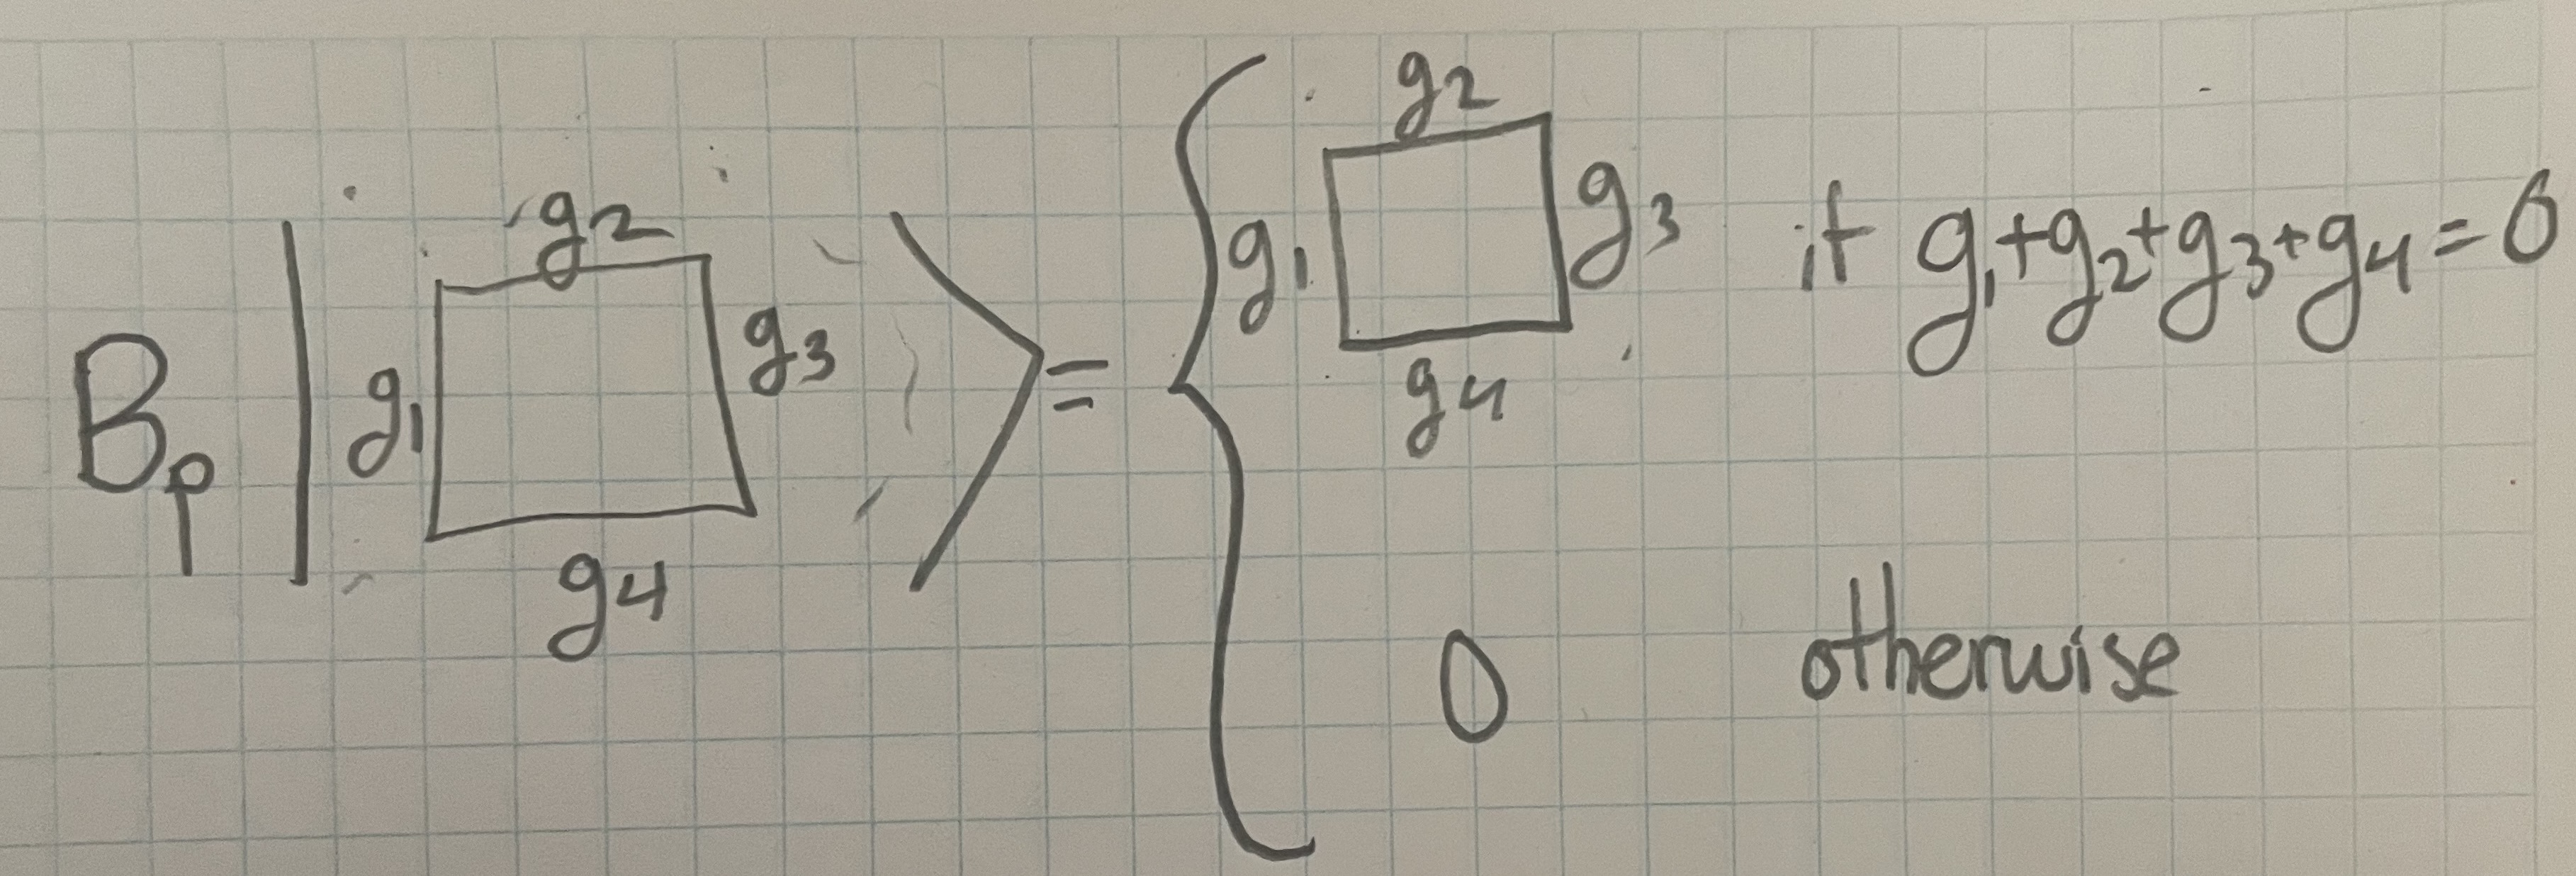
\includegraphics[scale=.04]{Bp-definition}
\end{center}
\end{figure}

In the present case, $B_p$ has a more workable expressing that is symmetric to our description of $B_p$. Define

\begin{align*}
\sigma_Z:\bC^2&\xrightarrow{}\bC^2.\\
\ket{0}&\mapsto \ket{0}\\
\ket{1}&\mapsto -\ket{1}
\end{align*}

Philosophically, it is useful to interpret $\sigma_Z$ as acting as $\ket{g}\mapsto \chi(g)\ket{g}$ where $\chi:\bZ_2\to\bC^\times$ is the unique nontrivial character of $\bZ_2$, $\chi(0)=1$, $\chi(1)=-1$. Since $\chi$ is a group isomorphism, for any $g_1,g_2,g_3,g_3\in G$ we have an equivalence

$$g_1+g_2+g_3+g_3=0 \iff \chi(g_1)\chi(g_2)\chi(g_3)\chi(g_4)=1.$$

Defining an auxillary $B_{p,1}$, we thus find the following expression for $B_p$:

\begin{align*}
B_{p,1}=\bigotimes_{\substack{\text{edges} \\ \text{bounding }p}}\sigma_Z, && B_p=\frac{1}{2}\left(I + B_{p,1}\right).
\end{align*}

For simplicity, we will often rewrite the Hamiltonian as

$$H=\frac{1}{2}\sum_{\text{vertices }v}(1-A_{v,1})+\frac{1}{2}\sum_{\text{plquettes }p}(1-B_{p,1}).$$

The matrices $\sigma_X$ and $\sigma_Z$ we defined are known as \textit{Pauli matrices}. They are extremely common across formulae in quantum mechanics - this is another reason that the toric code is so ammenable to error correction applications. The basic properties of these matrices are summarized below:

\begin{prop}$\,$
\begin{enumerate}[(a)]
\item The operators $\sigma_X$ and $\sigma_Z$ are simultaneously unitary and Hermitian;
\item $\sigma_X^2=\sigma_Z^2=I$;
\item $\sigma_X \sigma_Z = - \sigma_Z \sigma_X$;
\end{enumerate}
\end{prop}
\begin{proof}.[WORK: do proof]
\end{proof}

An important thing to note is that $A_{v,1}$ and $B_{p,1}$ commute, despite the fact that $\sigma_X$ and $\sigma_Z$ anticommute. The fact that they commute follows from Proposition [ref], though it fruitful to reavulate that proposition in this present context. The important fact is that given any vertex $v$ on the exterior of any face touching $p$,  there are an \textit{even number} of edges which both touch $v$ and bound $p$. Hence, the number of tensor factors in which $A_{v,1}$ and $B_{p,1}$ anticommute is even, and hence overall they commute.

The last step in reinterpreting our general theory of Kitaev quantum double models to the toric code is computing the ground space. We observe that since $\bZ_2$ is abelian acting by conjugation does nothing, and hence

$$\Hom(\pi_1(T^2,v), \bZ_2)/\left(\substack{\text{simultaneous} \\ \text{conjugation}}\right)=\Hom(\pi_1(T^2,v), \bZ_2).$$

Seeing as we are no longer modding out by conjucation, the group operation on $\bZ_2$ extends to a group operation on $\Hom(\pi_1(T^2,v), \bZ_2)$. Hence this space forms an abelian group, which we denote

$$H^1(T^2,\bZ_2)=\Hom(\pi_1(T^2,v), \bZ_2)=(\text{flat $\bZ_2$-colorings})/(\text{gauge transformations}).$$

[WORK: maybe set notation and write out four elements explicitely? Might be too much.]

This is the \textit{cohomology group of $T^2$ with coeffecients in $\bZ_2$}. Since $\pi_1(T^2,v)\cong \bZ^2$, we conclude that

$$H^1(T^2,\bZ_2)\cong \bZ_2^2.$$

Hence, we obtain the following:

\begin{prop} The $0$-eigenspace of $H$ is four dimensional. It is spanned by the vectors

$$\ket{C}=\frac{1}{\sqrt{|C|}}\sum_{\gamma\in C}\ket{\gamma}$$

for $C\in H^1(T^2,\bZ_2)$.
\end{prop}
\begin{proof}.[WORK: do proof]
\end{proof}

\subsubsection{Exact solution of the toric code}

When given a quantum system, the first thing to do with it is to \textit{solve it}. This means diagonalizing the Hamiltonian. In this case of the toric code, the diagonalization of $\cN$ is the direct sum decomposition

$$\cN = \bigoplus_{E\in \bR}\cN_{E}$$

where $\cN_{E}$ is the energy $E$ eigenspace,

$$\cN_{E}=\{\ket{\psi} | ,\, H\ket{\psi}= E \ket{\psi}\}.$$

Solving the toric code amounts to explicitely describing $\cN_E$ for each $E$. In particular, this means computing the dimension of each space. The Hamiltonian for the toric code is 

$$H=\sum_{v}(1-A_v)+\sum_{p}(1-B_p).$$

Since the $A_v$ and $B_p$ all commute with each other, they are \textit{simultaneously diagonalizable}. This is a huge help in our analysis. We introduce some notation to take advantage of this insight. We define a \textit{syndrome} on the toric code to be a map

$$\lambda: (\text{faces})\sqcup (\text{vertices})\xrightarrow{}\{\pm 1\}.$$

We define the syndrome $\lambda$ subspace of $\cN$ to be

$$\cN_{\lambda}=\{\ket{\psi}\in \cN | \,\, A_{v,1}\ket{\psi}=\lambda(v)\ket{\psi},\,\, B_{p,1}\ket{\psi}=\lambda(p)\ket{\psi}    \forall v,p\}$$

We define the energy $E_{\lambda}$ of a syndrome $\lambda$ by the formula

$$E_{\lambda}=\sum_{v}\frac{1}{2}(1-\lambda(v))+\sum_{p}\frac{1}{2}(1-\lambda(p)).$$

The fact that the operators $A_v$, $B_p$, and $H$ are simultaneously diagonalizable is codified in the following observations:

\begin{prop} We have that

\begin{align*}
\cN = \bigoplus_{\text{syndromes $\lambda$}} \cN_{\lambda}, && \cN_{E}=\bigoplus_{\substack{\text{syndromes $\lambda$}  \\ E_\lambda = E }  } \cN_{\lambda}.
\end{align*}

\end{prop}
\begin{proof} This follows immediately from the above discussion.
\end{proof}


We can now solve the toric code:

\begin{prop} We have that

\begin{equation*}
\dim(\cN_{\lambda}) = 
\begin{cases}
4 & \text{if }\prod_{v}\lambda(v) = \prod_{p}\lambda(p) = 1\\
0 & \text{otherwise.}
\end{cases}
\end{equation*}

\end{prop}
\begin{proof}.[WORK: do proof]
\end{proof}

\begin{cor} We have that

$$\dim (N_{E})=[WORK: write\,\, formula]$$
\end{cor}
\begin{proof} . [WORK: do proof]
\end{proof}

[WORK: this section will have some commentary about how Pauli operators are being used to fuse $X$-type and $Z$-type excitations. The way this commentary sounds should depend on the way the proof looks. I might want to include this lemma before the proof:

Given an edge $e$ in the lattice and an operator $U:\bC^2\to \bC^2$, denote by $(U)_e:\cN\to\cN$ the operator which applies $U$ on the tensor factor of $\bC^2$ at edge $e$. We compute the following:

\begin{lem} For any vertex $v$, edge $e$, plaquette $p$, we have

\begin{align*}
A_v  (\sigma_X)_e=(\sigma_X)e A_v, && B_p (\sigma_Z)_e=(\sigma_Z)e B_p,
\end{align*}

\begin{equation*}
A_v (\sigma_Z)_e=
\begin{cases}
- (\sigma_Z)_e A_v & \text{if $e$ touches $v$}\\
(\sigma_Z)_e A_V & \text{otherwise}
\end{cases}
\end{equation*}

and

\begin{equation*}
B_p (\sigma_X)_e=
\begin{cases}
- (\sigma_X)_e B_p & \text{if $e$ bounds $p$}\\
(\sigma_X)_e B_p & \text{otherwise}
\end{cases}
\end{equation*}


\end{lem}

]

\subsubsection{Toric code as a topologically ordered system}

.[WORK: prove that toric code satisfies axioms of TO.]

[WORK: This section will really dig into how the Pauli algebra acts on states]

[WORK: this section can also show that \textit{global} errors (e.g. $\sigma_X$ all the way around a torus) acts non-trivially. Maybe give a proof? Make a little quantum computer? If I do, I should reformulate it in in the ``adiabatically changing Hamiltonian" way to tie it into the way I talked about it in the introduction.]



\subsection{Anyons}

\subsubsection{Topological quantum information in excited states}

[WORK:

I've realized that I was wrong about anyons. I thought that they were localized excitations in a topologically ordered system. I was wrong. Anyons are \textit{stable} localized excitations in a topologically ordered system. This stability is what ensures that they will have a well-defined type. This correct definition should make the presentation a lot easier!
]

Let us recap our current picture of topological quantum information. We introduced topological order, and argued as a general principle that its ground states are invariant under local deformations. That is, if we start with a ground state in a topologically ordered system, apply some local operator, and then project back onto ground states, then we will get back to the state we started with up to some phase. This lets us store information in ground states. This information can be used as a place to store stable information, and can be acted on by global operators to perform computations such as in proposition [ref].

We now take this perspective to its logical extreme. The dimension of the ground state space depends only on the topological order of the system and the global topology of the physical space. For instance, toric code topological order on a torus will always have a four dimensional ground space, independent of system size or choice of microscopic lattice.

To make a computer, however, we need to be able to store arbitrarily large amounts of information. This means that either we will need to work with increasingly complex topological orders or increasingly complex surfaces. There are only a handful of topological orders known to be physically realizable, so working with increasinlgy complex topological orders is out of the question. Hence, once needs to work with increasingly complex surfaces. By working on high-genus surfaces, the ground state space can be made as large as possible. This gives the following picture for a topological quantum computer:

[WORK: add picture, a-la Freedman et al.]

This approach is potentially possible, and we will explore it more in section [ref]. However, no matter the implimentation it adds a great deal of complexity. Adding genus onto a computer chip is hard work. It would be much better to work with a state with the least complex topology possible, preferably a plane, sphere, or torus.

It is for this reason that we turn to a key idea in the theory of topological order: \textit{being careful, it is possible to store topologically protected information in the excited states of a topologically ordered system}.

[WORK: picture of spectrum diagram, with excited states boxed. ``Use these to store information!"]

Using the excited states of a topologically ordered system to store information comes with several obstacles:

\begin{enumerate}
\item It requires careful study. This isn't a fundamental problem, but it is relevant to us since we are about to embark on that study;
\item It requires a more powerful control over the topologically ordered system than working only with ground states. This can make the approach impossible in some physical systems;
\item It introduces non-topological local degrees of freedom. This non-topological information needs to be worked around so that proper fault-tolerant computations can be performed.
\end{enumerate}

We now recall our procedure for storing information in ground states. The key point is that we have a projector $\cP:\cN\xrightarrow{}\cN_{g.s.}$. This projector satisfies the relation that $\cP \cO \cP = \lambda\cdot \cP$ for any local operator $\cO$, for some $\lambda\in \bC$. Our physical picture for topological quantum computing is that we are continually measuring with respect to $\cP$, and hence constantly projecting into the ground space. The formula $\cP \cO \cP = \lambda \cdot \cP$ says that even if noise is applied between rounds of projection it is okay because our state will only change by a phase and hence will still store the same information.

As we leave the ground states, this protocol breaks down. We cannot continually project into ground states because that would destroy any information we are storing in excited states! If we don't have any sort of projector, however, errors will accumulate and we will lose all of the fault-tolerance of topological quantum computing. The answer is to find a new subspace $\cN' \subset \cN$ to store our information in, so that the orthogonal projector $\cP_{N'}: \cN \xrightarrow{} \cN'$ satisfies a formula similar to $\cP_{N'}\cO \cP_{N'}=\lambda\cdot \cP_{N'}$.

A first guess might to constantly measure with respect to the Hamiltonian, as before, and then project into a different energy eigenspace. We have a decomposition of $\cN$ by diagonalizing the Hamiltonian, $\cN=\bigoplus_{E\in \bR}\cN_{E}$. We can try storing our information in $\cN_{E}$, for some fixed $E>0$ independent of system size.

We demonstrate how this fails using the toric code, working with $E=4$. A generic state $\ket{\psi}$ in $\cN_{E=4}$ might look like this one:

[WORK: add picture, two sites with $X$-excitations, two sites with $Z$-excitations.]

The fact that there are exactly four terms in the Hamilotian that are violated corresponds exactly to the fact that the energy of the state is $E=4$. We now consider applying $\sigma_{X}$ to $\ket{\psi}$ at an edge adjacent to one of the $X$-excitations:

[WORK: add picture. Applying $(\sigma_X)_e$ moves the $X$-excitation.]

This new state with the $X$-excitation moved still has the same number of anyons, and hence $(\sigma_X)_e\ket{\psi}$ still leaves in $\cN_{E}$. Hence, $\cP_{E}(\sigma_X)_e\cP_{E}\ket{\psi}=(\sigma_X)_e\ket{\psi}$ does \textit{not} differ by a scalar. Even worse, despite the consant application of the projector $\cP_{E}$, local errors can accumate to become global errors. If we keep applying $\sigma_X$ on edges around some loop then this will never be detected by $\cP_{E}$, and this will be the same as acting by some non-trivial global operator. 

[WORK: add picture of local noise accumulating to be a global error.]

In summary, storing information in an excited energy level of a topologically ordered system does not result in information which is resistant to local noise. The problem is that the terms which violate the ground-state condition in the Hamiltonian can \textit{drift}, moving around the physical space in an uncrolled fashion without changing the energy of the system.

The solution to this problem is to \textit{constrain the drift}. This works as follows. We work in the Kitaev quantum double model based on some finite group $G$. Define a \textit{region} in a space to be a compact connected subset of it. Choose $n$ disjoint regions $R_1...R_n$ on the torus $T^2$. We define the space


$$\cN_{R_1,R_2... R_N}=\left\{\ket{\psi}\in \cN | \,\, A_v\ket{\psi}=B_p\ket{\psi}=\ket{\psi},\,\, \forall v,p\not\in \bigcup_{i=1}^n R_i \right\}.$$

This space consists of states which satisfy the condition to be in the ground state of $H=\sum_{v}(1-A_v)+\sum_p(1-B_p)$ outside of the regions  $R_1...R_n$, but is allowed to do whatever it wants within the regions. This is shown visually below:

[WORK: add picture]

The space $\cN_{R_1,R_2... R_N}$ contains all ground states, but also a large amount of excited states. The regions $R_1... R_n$ constrain the drift of excitations. To illustrate the power of this space, consider the example of the toric code. Suppose we have our same state $\ket{\psi}$ as below with energy $E=4$, but we consider it instead as a subspace of $\cN_{R_1,R_2,R_3,R_4}$ for some regions $R_1,...R_4$ containing the four excited operators. Applying $\sigma_X$ to an edge can still change the state, and so we don't have the formula $\cP_{N'}\cO \cP_{N'}=\lambda\cdot \cP_{N'}$, but local errors \textit{cannot} accumlate to become global errors! If the excited term starts to drift, it will eventually leave the region in started in and hence will no longer be in the subspace $\cN_{R_1,R_2,R_3,R_4}$, so projecting back into it will fix the error. This is shown pictorally below:

[WORK: add picture]

In this way, local operators can change the information stored in the system but it can only change it to a controlled degree. There is still global information within $\cN_{R_1,R_2... R_n}$ which is roughly invariant under local operators. Getting this global information out in such a way that the answer does not depend on whatever local operators are applied to the system is non-insurmountable challenge. This is the heart of point (3) in the obstacts of working with excited states: it introduces non-topological degrees of freedom which need to be worked around.

[WORK: notation is a bit junky because I'm working with $R_1,R_2... R_n$ all the time. It would be nicer in some ways if I worked with just one region $R$, and I dropped the condition that it be connected. This makes the definition of ``anyon" a bit more janky though. Not sure what to do.]

[WORK: So far I haven't defined what an anyon is for topological orders other than the KQDM. One easy way to do this is by putting some set $L$ of sites, choosing $d>0$, defining $\cN=\bigotimes_{\ell \in L}\bC^d$. Then we have $H=\sum_{i}H_i$, $[H_i,H_j]=0$, $H_i^2=1$, $H_i$ localized to some region $U_i$. This is a commuting local projector Hamiltonian. It is easy to define anyons in a model like this one. I'm not sure if this would be informative or distracting.

Actually, on second thought, something like this might actually be neccecary for the definition of TO. Hence, we might have it ready-to-use for this section.
]


\subsubsection{Definition and principles of anyons}

With the discussion in the previous section, we can start to see how our picture for topological quantum computing is similar to the picture for topological classcial computing described in chapter [ref]. The regions $R_1,R_2... R_n$ are localized regions of difference within a homogenous bulk. The bulk is homogenous because the wavefunction is groundstate of the Hamiltonian in those regions, and TQO-2 implies that all of these ground states are locally indistinugishable. The regions $R_1,R_2... R_n$ are different because they are allowed to be excited. Hence, the regions $R_1... R_n$ behave as \textit{quasiparticles}. We will show that these quasiparticles can be pair-created, braided, and fused, just like in topological classical computing. The major difference between our scheme for topological quantum computing and topological classical computing is that instead of our quasiparticles being defects in ordered media, they are localized excitations in a topological order. This leads us to the following definition:

\begin{defn} An \textit{anyon} is a localized excitation in a topologically ordered system.
\end{defn}

In our present context, this localization is best viewed not as an unavoidable physical reality but as a design decision for building a topological quantum computer. States $\ket{\psi}$ in topologically ordered systems have terms in the Hamiltonian that the violate and ones they don't. By circling regions around the terms they don't and constraining the excitation to those regions by repeatedly applying the projector $\cP_{\cN_{R_1,R_2... R_n}}$, we localize the excitation.

To store cohrent topological quantum information in anyons, there are a few key principles one must follow. The first principle is straightforward:

\begin{center}
\fbox{Anyons should be kept far apart}
\end{center}

This is motivated as follows. Suppose that the anyons were kept in close proximity to one another. Then local noise could affect two anyons at once:

[WORK: add picture of $R_1,R_2$ with some local noise operator $\cO$ touching both]

Our picture of our system is that there is contantly local noise being applied, and that we are contantly projecting into the space $\cN_{R_1,R_2... R_n}$. The fault-tolerant information we want to get at is exactly the information which is invariant under this noisy picture. That is, information which does not change when local operators from $\cN_{R_1,R_2... R_n}$ to itself is applied. We call this topological information.

Some of this topological information can be measured using local observables. Because physics is local, any realistic observable should be local. Suppose we have a local Hermitian operator $\pi: \cN_{R_1,R_2... R_n}\to \cN_{R_1,R_2... R_n}$ which commutes with every noise operator $\cN_{R_1,R_2... R_n}\to \cN_{R_1,R_2... R_n}$. Then $\pi$ can be physically measured \textit{and} the result of that measurement is invariant under noise. Hence, it gives topological information. We all such observables $\pi$ which are locally supported and commute with every noise operator \textit{local topological observables}. We image that the outcomes of local topological measurements are readily available to experimenters - they can be measured with physical devices in a way that does not depend on noise.

This allows us to break-down the information in our system:

[WORK:

Four-square diagram for information in $\cN_{R_1,R_2... R_n}$.

Collumns: measurable by local topological observables. (yes/no)

Rows: invariant under local noise. (yes/no)

C-yes R-no: Impossible.

C-no R-no: Non-topological information.

C-yes R-yes: Classical information / local topological information

C-no R-no: Topological quantum information / global information 

Add little arrows going to each box explaining it.
]


[WORK:

Measuring under all topological observables should be called a ``topological charge measurement". This leads to harmony with the language used in the MTC section.

]
We now break down this general picture into exact mathematical statements.

[WORK: at this point I need to read Kitaev's arguement in more detail.

The first step is to go $\cN_{R_1,... R_n}=\bigoplus_{i=1}^{N}\cN_{i}$ where $\cN_i$ indexes over classical information. This is easy. The non-trivial step is to observe that there exists some finite set $\cL$ such that the terms $\cN_i$ can be rearranged as 

$\cN_{R_1,... R_n}=\bigoplus_{(A_i)_{i=1}^n\in \cL^n}\cN_{A_1,A_2... A_n}.$

Each $A_i$ is the result of a measurement localized around $R_i$. The set $\cL$ is the set of anyon types, and given some state $\ket{\psi}\in \cN_{A_1,A_2... A_n}$, we call $A_i$ the type of the anyon at $R_i$. Anyon types = topological classical information.

Now, the next step is to observe that there is a non-canonical tensor decomposition


$$
\cN_{A_1,A_2... A_n}=\cN^{loc}_{A_1,A_2... A_n}\otimes \cN^{top}_{A_1,A_2... A_n}
$$

of $\cN_{A_1,A_2... A_n}$ into a local part and a topological part. It satisfies the condition that every local noise operator $\cO$ on $\cN_{A_1,A_2... A_n}$ can be decomposed as $\cO=\cO'\otimes \id$, and hence the information in the topological part remains unchanged. Moreover, it is maximal subject to this condition. Moreover, we have a splitting

$$\cN^{loc}_{A_1,A_2... A_n}=\cN^{loc}_{A_1}\otimes \cN^{loc}_{A_2}...\otimes \cN^{loc}_{A_n}.$$


Information of which direct summand I'm in = topological classical information

Information left over = tensor product of local and topological. Cannot be distinguished by the non-canonical nature of this tensor decomposition. Needs subtle techniques (i.e. fusion of anyons) to be measured. It would be fantastic if all of this could be written up correctly and codified into propositions.
]


[WORK: I want to get to the fact that anyons are moved by unique operators, and hence we can ignore the specific choice of operator and just move the anyons.]

[WORK: The notion of anyon types is explaned well by Kawagoe and Levin \cite{kawagoe2020microscopic}:

quote: We begin with the idea of “anyon types.” ... anyon excitation of type a, type b,
type c, etc.]

\subsubsection{Anyons in the toric code}

[WORK: do it first with toric code. Everything is painfully simple and obvious here.

The problem is that adding more anyons does not encode more information, so its hard to get the points of TQC across.

Hopefully this is a very short subsection.]

\subsubsection{Anyons in discrete gauge theory}

[WORK:

Here we go from KQDM to $G$-crossed $G$-representations. By the end we should have the category $\fD(G)$ as a set, with morphisms motivated.

A lot of the intricate setup has been done in the previous sections, so I think this can be relatively contained. It would be nice to have proofs. Even if this section is more intricate that should be included in most lectures series, I'd say its nice to have nonetheless as a reference.
]

$\newline$
\fbox{\parbox{\dimexpr\linewidth-2\fboxsep-2\fboxrule\relax}{

\begin{center}
\textbf{History and further reading:}\\
\end{center}

The term topological order was first used in 1972 by Kosterlitz and Thouless to describe topological classical systems of the sort discussed in Chapter [ref] \cite{kosterlitz2018ordering} . The term has since evolved, and was re-coined in 1989 by Xiao-Gang Wen to describe the sort of topological classical systems defined in this chapter \cite{wen1989vacuum}.

$\newline$
The history anyons is distinct from the history of topological order. It was first noted in 1976  in a paper of Leinass and Myrheim that the classification of particles in terms of fermions and bosons broke down in two dimensions \cite{leinaas1977theory}. The subject of anyons was then taken over by Wilczek who published a series of seminal papers on the topic \cite{wilczek1982magnetic, wilczek1982quantum, arovas1984fractional}. It was in these papers that Wilczek observed that anyons were present in the quantum Hall effect, and hence connected the theory of anyons and topological order together.

[WORK: what is the history of gauge theory, and when was it introduced to the picture? A great reference is the de Wild Propitius and Bais survey. Also should mention Kitaev's paper again.]

}}


$\newline\newline$

\large \textbf{Exercises}:\normalsize

\begin{enumerate}[\thesection .1.]

\item For vertices $v$ and plaquettes $p$, define

\begin{align*}
A'_{v,1}=\bigotimes_{\substack{\text{edges} \\ \text{touching }v}}\sigma_Z, && A'_v=\frac{1}{2}\left(I + A'_{v,1}\right),
\end{align*}

\begin{align*}
B'_{p,1}=\bigotimes_{\substack{\text{edges} \\ \text{bounding }p}}\sigma_X, && B'_p=\frac{1}{2}\left(I + B'_{p,1}\right),
\end{align*}

and

$$H'=\sum_{\text{vertices }v}(1-A'_v)+\sum_{\text{plaquettes }p}(1-B'_p).$$

Define $M:\bC^2\to \bC^2$ by $M(\ket{0})=\frac{1}{\sqrt{2}}(\ket{0}+\ket{1})$ and $M(\ket{1})=\frac{1}{\sqrt{2}}(\ket{0}-\ket{1})$. Show that

$$\sigma_X=M\sigma_ZM^{-1},\,\, \sigma_{Z}=M\sigma_X M^{-1},$$

and show that $H$ and $H'$ are similar in the sense that $H'=MHM^{-1}$. Use this to conclude that all basis independent properties of the toric code are formally symmetric by replacing $\sigma_X$ with $\sigma_Z$. For example, conclude that the codespace of $H'$ is 4 dimensional.

\end{enumerate}